\documentclass[12pt,oneside,letterpaper]{report}

% --- Packages ---
\usepackage[top=1.5in, left=1.5in, bottom=1in, right=1in]{geometry}
\usepackage{setspace}
\usepackage{titlesec}
\usepackage{tocloft}
\usepackage{etoolbox}
\usepackage{hyperref}
\usepackage{graphicx}
\usepackage{amsmath}
\usepackage{amssymb}
\usepackage{booktabs}
\usepackage{caption}
\usepackage{subcaption}
\usepackage{multirow}
\usepackage{array}
\usepackage{xcolor}
\usepackage{microtype}
\usepackage{float}

% --- Prevent text overflowing right margin ---
\setlength{\emergencystretch}{3em}
\hbadness=10000

% --- TOC/List Formatting ---
\setlength{\cftbeforechapskip}{1em}
\setlength{\cftbeforesecskip}{1em}

% --- Figure path ---
\graphicspath{{out/figures/}}

% --- Shorthand macros ---
\newcommand{\dH}{$\Delta H$}
\newcommand{\Tm}{$T_m$}
\newcommand{\dG}{$\Delta G_{37}$}
\newcommand{\dS}{$\Delta S$}

\begin{document}

% ---------------------------------------------------------
% PRELIMINARY PAGES
% ---------------------------------------------------------
\pagenumbering{roman}
\setcounter{page}{1}

% 1. TITLE PAGE
\thispagestyle{empty}
\begin{center}
    UNIVERSITY OF CALIFORNIA \\
    RIVERSIDE \\
    \vspace{1in}
    Inductive Biases in Representation Learning for DNA Thermodynamic Property Prediction \\
    \vspace{1in}
    A Thesis submitted in partial satisfaction \\
    of the requirements for the degree of \\
    \vspace{0.5in}
    Master of Science \\
    \vspace{0.1in}
    in \\
    \vspace{0.1in}
    Computer Science \\
    \vspace{0.5in}
    by \\
    \vspace{0.5in}
    Anant Shrenik Patil \\
    \vspace{0.5in}
    June 2026
\end{center}
\vfill
\noindent
Thesis Committee: \\
\hspace*{0.5in}Dr.\ Philip Brisk, Chairperson \\
\hspace*{0.5in}Dr.\ William Grover \\
\hspace*{0.5in}Dr.\ Tao Jiang
\clearpage

% 2. COPYRIGHT PAGE
\thispagestyle{empty}
\vspace*{7.5in}
\begin{center}
    Copyright by \\
    Anant Shrenik Patil \\
    2026
\end{center}
\clearpage

% 3. SIGNATURE APPROVAL PAGE
\thispagestyle{empty}
\vspace*{0.5in}
\noindent The Thesis of Anant Shrenik Patil is approved:

\vspace{0.55in}
\noindent \makebox[0.20\textwidth]{} \makebox[0.75\textwidth]{\hrulefill}

\vspace{0.55in}
\noindent \makebox[0.20\textwidth]{} \makebox[0.75\textwidth]{\hrulefill}

\vspace{0.55in}
\noindent \makebox[0.20\textwidth]{} \makebox[0.75\textwidth]{\hrulefill}\\[-4pt]
\makebox[0.20\textwidth]{} \makebox[0.70\textwidth][r]{Committee Chairperson}

\vspace{1.0in}
\begin{center}
    University of California, Riverside
\end{center}
\clearpage

% 4. ACKNOWLEDGEMENTS
\setcounter{page}{4}
\begin{center}
    ACKNOWLEDGMENTS
\end{center}
\vspace{0.5in}
\setstretch{2.0}

I want to express my sincere gratitude to Professor Philip Brisk for giving me the opportunity to pursue this research under his supervision. The guidance, support, and computational resources he provided throughout this project made all of it possible. I am grateful for that.

\clearpage

% 5. ABSTRACT
\begin{singlespace}
\begin{center}
    ABSTRACT OF THE THESIS \\
    \vspace{0.2in}
    Inductive Biases in Representation Learning for DNA Thermodynamic Property Prediction \\[0pt]
    by \\[0pt]
    Anant Shrenik Patil \\[0pt]
    Master of Science, Graduate Program in Computer Science \\[0pt]
    University of California, Riverside, June 2026 \\[0pt]
    Dr.\ Philip Brisk, Chairperson
\end{center}
\end{singlespace}
\vspace{0.5in}
\setstretch{2.0}

Predicting the thermodynamic properties of short DNA oligonucleotides, specifically, melting temperature ($T_m$), enthalpy ($\Delta H$), and Gibbs free energy at 37$^\circ$C ($\Delta G_{37}$), is a central problem in computational biophysics with applications in PCR primer design~\cite{santalucia1998}, CRISPR guide RNA engineering~\cite{doench2016}, and DNA nanotechnology~\cite{seeman2018}. The classical nearest-neighbor (NN) model of SantaLucia and Hicks provides accurate predictions for standard Watson-Crick duplexes but struggles with the full diversity of hairpin topologies encountered in synthetic library experiments.

This thesis asks a specific question about representation learning: does the choice of neural network architecture, and the inductive bias it encodes, affect the ability to learn DNA thermodynamics from data? Using the Array Melt dataset of approximately 30,000 DNA sequences from Greenleaf et al.\ (2025), I train and evaluate six architectures, each embodying a distinct geometric prior: a Graph Neural Network (GNN), a one-dimensional CNN (1D CNN), a novel two-dimensional Folded Ladder CNN (2D CNN), a Structure-Aware Transformer (SAT), a Physics-Informed Neural Network (PINN), and a Hybrid CNN-RNN.

All models are trained exclusively on the Array Melt hairpin partition and evaluated for generalization on two external duplex datasets: 348 literature UV melting sequences (\texttt{lit\_uv}) and 2,775 mismatch-containing duplex sequences from Oliveira et al.\ (\texttt{ov}). The Hybrid CNN-RNN achieves the best in-distribution performance ($T_m$ MAE = 1.53$^\circ$C) followed closely by the 2D CNN (1.57$^\circ$C), while the GNN performs worst in-distribution (3.28$^\circ$C). Out-of-distribution on the UV-melt data, the ranking inverts: the GNN generalizes best (5.59$^\circ$C on \texttt{lit\_uv}), while the 2D CNN generalizes worst (9.95$^\circ$C). On the mismatch duplex dataset, the GNN (5.27$^\circ$C) is the only model that generalizes consistently, outperforming the classical SantaLucia nearest-neighbor model (9.94$^\circ$C), which systematically overpredicts $T_m$ because it cannot account for mismatch destabilization. Notably, all six deep learning models underperform the classical SantaLucia model (1.85$^\circ$C) on the perfectly complementary \texttt{lit\_uv} evaluation, suggesting that high in-distribution accuracy does not imply learning of true thermodynamic physics.

These results show that inductive biases aligned with the training measurement apparatus improve in-distribution performance but hinder generalization, while biases grounded in physical molecular structure, such as the GNN's explicit base-pair graph or the PINN's thermodynamic loss, generalize more robustly across experimental conditions.

\clearpage

% 6. TABLE OF CONTENTS, FIGURES, TABLES
\begin{singlespace}
\tableofcontents
\clearpage
\listoffigures
\clearpage
\listoftables
\end{singlespace}
\clearpage

% ---------------------------------------------------------
% MAIN BODY
% ---------------------------------------------------------
\pagenumbering{arabic}
\setcounter{page}{1}
\setstretch{2.0}

% =========================================================
\chapter{Introduction}
% =========================================================

\section{Motivation}

Every time a biologist designs a PCR primer, synthesizes a CRISPR guide RNA, or builds a DNA origami structure, they are implicitly relying on a prediction: will this short DNA sequence fold into the intended structure, and how stable will it be? The thermodynamic properties of DNA oligonucleotides (how much heat they release when hybridizing, \dH; the temperature at which half the population is folded, \Tm; and the free energy of the folded state, \dG) are the numbers that answer those questions.

For decades, these predictions came from a single source: the nearest-neighbor (NN) thermodynamic model developed by SantaLucia and collaborators~\cite{santalucia1998,santalucia2004}. This model decomposes the free energy of a duplex or hairpin into a sum of contributions from adjacent base-pair stacks, using experimentally measured parameters for each of the ten unique dinucleotide combinations. It is elegant, interpretable, and remarkably accurate for standard DNA duplexes. But it is fundamentally limited to the structural motifs for which parameters have been measured, it assumes that thermodynamic contributions are strictly additive between neighbors, and it cannot easily capture unusual loop geometries, terminal mismatch effects, or the complex dependence of hairpin stability on loop sequence.

In 2025, Greenleaf and colleagues published a dataset of approximately 30,872 DNA thermodynamic measurements collected in a single experiment using a high-throughput microarray platform~\cite{greenleaf2025}. For the first time, this made it possible to train a deep learning model on a large, controlled, uniform dataset of DNA hairpin thermodynamics. Their best model, a Graph Neural Network (GNN), reduced the NN model's error on held-out sequences from about 0.4~kcal/mol to 0.18~kcal/mol on $\Delta G_{37}$, a meaningful improvement.

This raises an immediate follow-up question that the original paper does not fully address: is the GNN the right model for this problem? Or would a different neural network architecture, one that encodes different assumptions about the structure of the input, do better?

\section{The Central Question}

This thesis is fundamentally about representation learning. Given the same sequence and secondary structure string, different architectures will process the input in fundamentally different ways:

\begin{itemize}
    \item A \textbf{Graph Neural Network} treats each nucleotide as a node and the backbone bonds and hydrogen bonds as edges, building a representation that is invariant to the ordering of nodes.
    \item A \textbf{1D Convolutional Neural Network} treats the sequence as a one-dimensional signal of length $L$, applying learned filters that detect local subsequence motifs independent of their position.
    \item A novel \textbf{2D Folded Ladder CNN} (the principal original contribution of this thesis) folds the hairpin sequence at its loop midpoint into a two-dimensional matrix, placing paired bases in adjacent rows so that Watson-Crick base-stacking interactions become spatially local in two dimensions.
    \item A \textbf{Structure-Aware Transformer} injects the structural adjacency matrix directly into the self-attention mechanism.
    \item A \textbf{Physics-Informed Neural Network} modifies the loss function to enforce thermodynamic consistency between predicted $\Delta H$ and $T_m$.
    \item A \textbf{Hybrid CNN-RNN} processes the sequence through both a 2D CNN branch and a bidirectional GRU branch simultaneously.
\end{itemize}

Each of these choices embeds a different inductive bias --- a different set of assumptions about what structure in the input is relevant to the output. The question I investigate is: which bias best captures the thermodynamics of DNA oligonucleotides?

\section{Contributions}

The main contributions of this thesis are:

\begin{enumerate}
    \item The design and evaluation of the \textbf{2D Folded Ladder encoding} for DNA hairpin sequences, a novel representation that places complementary paired bases in adjacent spatial rows to align the architectural bias of 2D convolutions with base-pair stacking physics.
    \item A \textbf{systematic comparison of six neural network architectures} on the Array Melt dataset, using identical training protocols, data splits, and evaluation metrics for fair comparison.
    \item An \textbf{out-of-distribution generalization evaluation} on 348 classical UV-melt duplex sequences, revealing a striking inversion: models that perform best in-distribution generalize worst to the external dataset.
    \item A \textbf{comparison against the SantaLucia classical baseline} on the out-of-distribution evaluation, showing that all deep learning models trained on array hairpin data underperform the physical model on external duplex data.
\end{enumerate}

\section{Thesis Organization}

Chapter~2 provides the necessary background on DNA thermodynamics, the Array Melt dataset, and the concept of inductive biases in deep learning. Chapter~3 reviews related work in the literature. Chapter~4 describes the methods: the six model architectures, the training protocol, and the evaluation design. Chapter~5 presents the in-distribution results. Chapter~6 presents the generalization results and discusses what they mean. Chapter~7 concludes the thesis and outlines directions for future work.

% =========================================================
\chapter{Background}
% =========================================================

\section{DNA Structure and Secondary Structure}

DNA is a polymer of four nucleotide bases --- adenine (A), thymine (T), guanine (G), and cytosine (C) --- connected by a phosphodiester backbone. Under physiological conditions, single-stranded DNA can fold onto itself to form \textit{secondary structures}: short double-stranded stems held together by Watson-Crick base pairs (A--T and G--C) connected by single-stranded loops. These are called \textbf{hairpins}~\cite{zuker2003}. Alternatively, two complementary strands can hybridize to form a \textbf{duplex}.

Secondary structure is commonly written in dot-bracket notation: parentheses denote paired bases (``('' on the 5$'$ side, ``)'' on the 3$'$ side), and dots denote unpaired loop positions. For example, the structure \texttt{(((....)))} describes a hairpin with a 3-base-pair stem and a 4-nucleotide loop.

\section{Thermodynamic Parameters}

The stability of a DNA secondary structure is characterized by three thermodynamic quantities derived from a two-state folding model~\cite{santalucia1998}:

\begin{itemize}
    \item $\Delta H$ (enthalpy, kcal/mol): the heat released during hybridization. More negative values indicate stronger binding.
    \item $T_m$ (melting temperature, $^\circ$C): the temperature at which half the population is in the folded state. Depends on both $\Delta H$ and $\Delta S$.
    \item $\Delta G_{37}$ (Gibbs free energy at 37$^\circ$C, kcal/mol): the net free energy of folding at body temperature, derived as:
\end{itemize}

\begin{equation}
    \Delta G_{37} = \Delta H - (310.15\,\text{K}) \cdot \Delta S
    \label{eq:gibbs}
\end{equation}

The melting temperature is related to $\Delta H$ and $\Delta S$ by:

\begin{equation}
    T_m = \frac{\Delta H}{\Delta S + R \ln(C_T / N)} - 273.15
    \label{eq:tm}
\end{equation}

where $R = 1.987\,\text{cal/(mol·K)}$ is the gas constant, $C_T$ is the total strand concentration in molar, and $N = 1$ for self-complementary or hairpin sequences, $N = 4$ for non-self-complementary duplexes. In this thesis, I predict $\Delta H$ and $T_m$ directly and derive $\Delta G_{37}$ analytically using Equation~\ref{eq:gibbs}.

\section{The Nearest-Neighbor Model}

The dominant classical approach to DNA thermodynamics is the nearest-neighbor (NN) model~\cite{santalucia1998,santalucia2004}. The model assumes that the free energy of a duplex or hairpin stem is the sum of contributions from each adjacent pair of stacked base pairs (``dinucleotide stacks''):

\begin{equation}
    \Delta H = \sum_{i=1}^{n-1} \Delta H_{X_i X_{i+1}} + \Delta H_{\text{init}}
    \label{eq:nn}
\end{equation}

where $X_i X_{i+1}$ denotes the dinucleotide stack at position $i$, and $\Delta H_{\text{init}}$ is an initiation correction that depends on the terminal base pairs. There are 10 unique Watson-Crick dinucleotide stacks; SantaLucia and Hicks (2004) provide experimentally measured $\Delta H$ and $\Delta S$ for each, enabling prediction of $T_m$ via Equation~\ref{eq:tm}.

The NN model works well for standard duplexes under standard ionic conditions, but it has important limitations discussed in Chapter~3.

\section{The Array Melt Dataset}

The experimental foundation of this thesis is the Array Melt dataset from Greenleaf et al.\ (2025)~\cite{greenleaf2025}. The Greenleaf lab developed a microarray-based platform, also called Array Melt, that measures the thermodynamic properties of tens of thousands of DNA sequences simultaneously on a repurposed Illumina sequencing flow cell. Key details:

\begin{itemize}
    \item Short DNA hairpin sequences (11--24 nucleotides) are synthesized on a chip at densities of over 100,000 unique sequences.
    \item Melt curves are collected by temperature-controlled fluorescence imaging, yielding $\Delta H$ and $T_m$ for each sequence under controlled ionic conditions.
    \item The resulting dataset contains approximately 30,872 hairpin sequences, referred to in the data files as the Array Melt partition (\texttt{arr}).
\end{itemize}

In addition to the Array Melt hairpin data, the combined dataset released by Greenleaf et al.\ includes three external sets:
\begin{itemize}
    \item The Oliveira et al.\ duplex melting dataset (\texttt{ov}): 2,775 duplex sequences with single, double, and triple mismatches, with $T_m$ only~\cite{oliveira2020}.
    \item A cloud-lab UV melting validation set (\texttt{uv}): 19 hairpin sequences with both $\Delta H$ and $T_m$, measured at Emerald Cloud Lab to cross-validate the Array Melt method.
    \item The literature UV melting dataset (\texttt{lit\_uv}): 384 Watson-Crick pairing DNA duplex sequences compiled from multiple published UV melting studies~\cite{greenleaf2025}, with measured $T_m$ values collected under varying ionic conditions. After removing entries with missing values, 348 sequences are used in this thesis.
\end{itemize}

In this thesis, all models are trained on the Array Melt partition (\texttt{arr}) only. The literature UV melting dataset (\texttt{lit\_uv}) serves as the primary out-of-distribution generalization benchmark, since it represents a different molecule type (duplexes vs.\ hairpins), a different measurement technology (classical UV melting vs.\ array fluorescence), and different ionic conditions.

\section{Inductive Biases in Deep Learning}

Every machine learning model contains an \textit{inductive bias} --- a set of assumptions built into the architecture that determines how it generalizes from training examples to new ones. The choice of inductive bias is arguably the most consequential design decision in deep learning, particularly when the training and test data come from different distributions.

Bronstein et al.\ (2021) provided a rigorous framework for understanding inductive biases through the lens of symmetry groups~\cite{bronstein2021}. They showed that most successful deep learning architectures can be understood as implementing equivariance to a specific symmetry group:

\begin{itemize}
    \item \textbf{1D CNNs}: equivariant to the translation group $T(1)$ along the sequence axis. The same filter is applied at every position, so the model responds identically to a motif regardless of where it appears.
    \item \textbf{2D CNNs}: equivariant to $T(2)$, the 2D translation group. The same local filter fires wherever a spatial pattern appears in the image.
    \item \textbf{GNNs}: equivariant to the permutation group $S_n$ over nodes. The prediction is invariant to the arbitrary numbering of nodes (nucleotides).
\end{itemize}

The design principle is: if the underlying physical problem has a known symmetry, the architecture should be built to respect that symmetry. For DNA thermodynamics, different symmetries are appropriate depending on how the molecule is represented --- and this is precisely the question this thesis investigates.

% =========================================================
\chapter{Related Work}
% =========================================================

\section{Convolutional Neural Networks for Genomic Sequences}

The application of CNNs to DNA sequences was established by DeepBind~\cite{alipanahi2015}, which showed that a 1D convolutional architecture trained on raw one-hot sequence data could learn sequence-specific binding specificities competitive with, and often better than, support vector machines with hand-crafted k-mer features. The key insight was that 1D convolutions act as learned position-weight matrices: each filter detects a specific subsequence motif regardless of where it appears in the input sequence.

DeepSEA~\cite{zhou2015} extended this to predicting chromatin accessibility and transcription factor binding across 919 genomic features from 1 kb DNA windows. Both models use global max-pooling as the readout function, which detects whether a motif is present anywhere in the window. For thermodynamic regression over short sequences, where every position matters, adaptive average pooling is more appropriate than max-pooling.

More recently, DeepSTABp~\cite{deepstabp} applied recurrent and convolutional architectures to protein melting temperature prediction, showing that sequential models can capture length-dependent thermal stability effects. For DNA, analogous effects are expected: longer stems are generally more stable, and A/T-rich regions lower $T_m$ while G/C-rich regions raise it.

\section{Graph Neural Networks for Molecules}

The application of GNNs to molecular property prediction was systematized by the Message Passing Neural Network (MPNN) framework of Gilmer et al.~\cite{gilmer2017}. In the MPNN formalism, each atom (node) accumulates messages from its bonded neighbors and updates its representation. After $k$ rounds of message passing, the representation of each node reflects its $k$-hop neighborhood. A permutation-invariant readout function (sum, mean, or Set2Set) produces a graph-level representation for prediction.

Applied to DNA, the Greenleaf GNN uses a GraphTransformer~\cite{shi2021} architecture (implemented as \texttt{TransformerConv} in PyTorch Geometric), which extends the MPNN by using multi-head attention to compute message weights:

\begin{equation}
    \mathbf{h}_v^{(t+1)} = \sum_{w \in \mathcal{N}(v)} \alpha_{vw} \left( \mathbf{W}_V \mathbf{h}_w^{(t)} + \mathbf{W}_E \mathbf{e}_{vw} \right)
    \label{eq:graphtransformer}
\end{equation}

where $\alpha_{vw}$ are softmax-normalized attention weights and $\mathbf{e}_{vw}$ is the edge feature vector (backbone or hydrogen bond type). Graph-level aggregation uses Set2Set pooling~\cite{vinyals2016}, which is an LSTM-based attention mechanism that produces a fixed-length graph embedding invariant to node ordering.

\section{Attention Mechanisms and Transformers for Biological Sequences}

Following the success of the Transformer architecture in NLP~\cite{vaswani2017}, several works have applied transformer-style self-attention to DNA and RNA sequences:

\begin{itemize}
    \item \textbf{DNABERT}~\cite{dnabert2021}: a BERT-style model pretrained on $k$-mer tokenized genomic sequences for regulatory element prediction.
    \item \textbf{Nucleotide Transformer}~\cite{nucleotidetransformer2023}: a large foundation model for human genomics trained on 850 million nucleotides.
    \item \textbf{RNA-FM}~\cite{rnaFM2022}: a foundation model for RNA sequences and structures.
\end{itemize}

These models target long genomic sequences (hundreds to thousands of nucleotides). For the short oligonucleotides in the Array Melt dataset (11--24 nt), the global attention mechanism is arguably unnecessary --- the entire sequence fits within a small local window. This motivated the Structure-Aware Transformer in this thesis, which focuses the attention mechanism on structurally relevant positions rather than computing full all-pairs attention.

\section{Physics-Informed Neural Networks}

Physics-Informed Neural Networks (PINNs), introduced by Raissi et al.~\cite{raissi2019}, incorporate known physical laws into the neural network loss function as soft constraints, penalizing predictions that violate the equations of physics. The approach has been applied broadly in fluid mechanics, materials science, and heat transfer.

For DNA thermodynamics, the relevant physical law is the relationship between $\Delta H$, $\Delta S$, and $T_m$ (Equation~\ref{eq:tm}). A physics-informed approach to DNA thermodynamics prediction would have the model predict $\Delta H$ and $\Delta S$ separately, compute $T_m$ analytically inside the forward pass, and penalize thermodynamic violations in the loss. To my knowledge, this approach has not been previously applied to oligonucleotide thermodynamics prediction.

\section{Hybrid CNN-RNN Architectures}

Combining CNNs and RNNs in a single model has been explored for several biological sequence tasks. For DNA melting, there is a natural dual-modality interpretation: the \textit{static structure} (which bases are paired, captured by the 2D Folded Ladder CNN) and the \textit{sequential unzipping process} (the order in which base pairs open during melting, captured by a recurrent network along the sequence) are both physically meaningful. DeepMEL~\cite{deepmel2020} used a similar CNN-RNN hybrid for chromatin accessibility from sequence, showing complementary feature extraction between local convolutions and sequential RNN context.

% =========================================================
\chapter{Methods}
% =========================================================

\section{Data and Preprocessing}

All models in this thesis are trained and evaluated on the Array Melt dataset from Greenleaf et al.~\cite{greenleaf2025}. The training set consists of 25,009 Array Melt hairpin sequences (\texttt{arr}, after removing 2,721 sequences with NaN measurements), with a validation set of 1,385 sequences and a test set of 1,395 sequences, all from the \texttt{arr} partition. The literature UV melting dataset (\texttt{lit\_uv}, 348 duplex sequences) is held out entirely and used only for out-of-distribution evaluation.

The targets $\Delta H$ and $T_m$ are normalized to the range $[0, 1]$ using the training-set minimum and maximum:

\begin{equation}
    \hat{y} = \frac{y - y_{\min}}{y_{\max} - y_{\min}}
    \label{eq:norm}
\end{equation}

Normalization statistics are computed from the training set only and applied to validation, test, and OOD evaluation sets. $\Delta G_{37}$ is never predicted directly; it is always derived from predicted $\Delta H$ and $T_m$ using Equation~\ref{eq:gibbs}.

\section{Model Architectures}

Each subsection below describes one architecture's input encoding, inductive bias, and prediction head, accompanied by a block diagram.

\subsection{E0: Graph Neural Network (GNN)}

\begin{figure}[H]
    \centering
    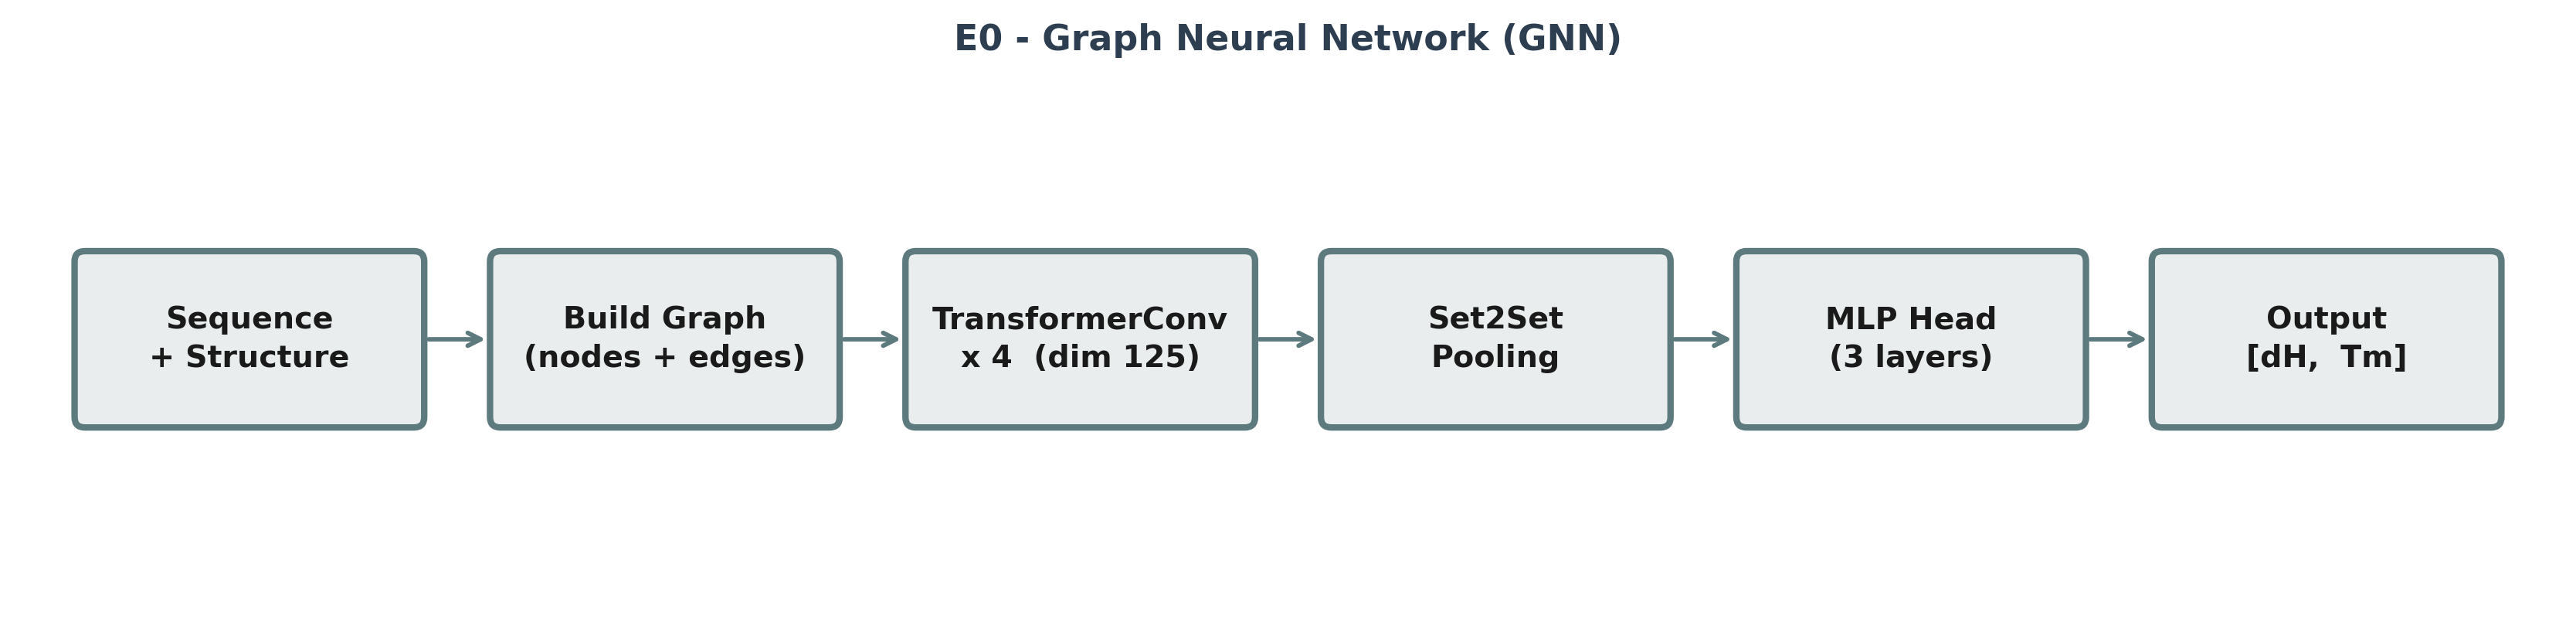
\includegraphics[width=\textwidth]{arch_e0_gnn.png}
    \caption{E0 --- Graph Neural Network (GNN). Sequence and dot-bracket structure are converted to a graph (nodes: nucleotides; edges: backbone and hydrogen bonds). Four \texttt{TransformerConv} layers propagate information across the graph, followed by Set2Set pooling and a 3-layer MLP predicting $[\hat{\Delta H}, \hat{T}_m]$.}
    \label{fig:arch_gnn}
\end{figure}

The GNN baseline replicates the architecture from Greenleaf et al.~\cite{greenleaf2025} using PyTorch Geometric. Each DNA sequence is converted to a graph where:

\begin{itemize}
    \item \textbf{Nodes}: one node per nucleotide, with a 4-dimensional one-hot feature vector (A, T, C, G).
    \item \textbf{Edges}: bidirectional backbone bonds (5$'$→3$'$ and 3$'$→5$'$) and bidirectional hydrogen bonds derived from the dot-bracket structure, each with a 3-dimensional one-hot edge feature vector.
\end{itemize}

The architecture consists of four \texttt{TransformerConv} layers with hidden dimension 125, followed by Set2Set pooling (10 processing steps), and a 3-layer MLP prediction head. The output is two values: normalized $[\hat{\Delta H}, \hat{T}_m]$.

\subsection{E1: One-Dimensional CNN (1D CNN)}

\begin{figure}[H]
    \centering
    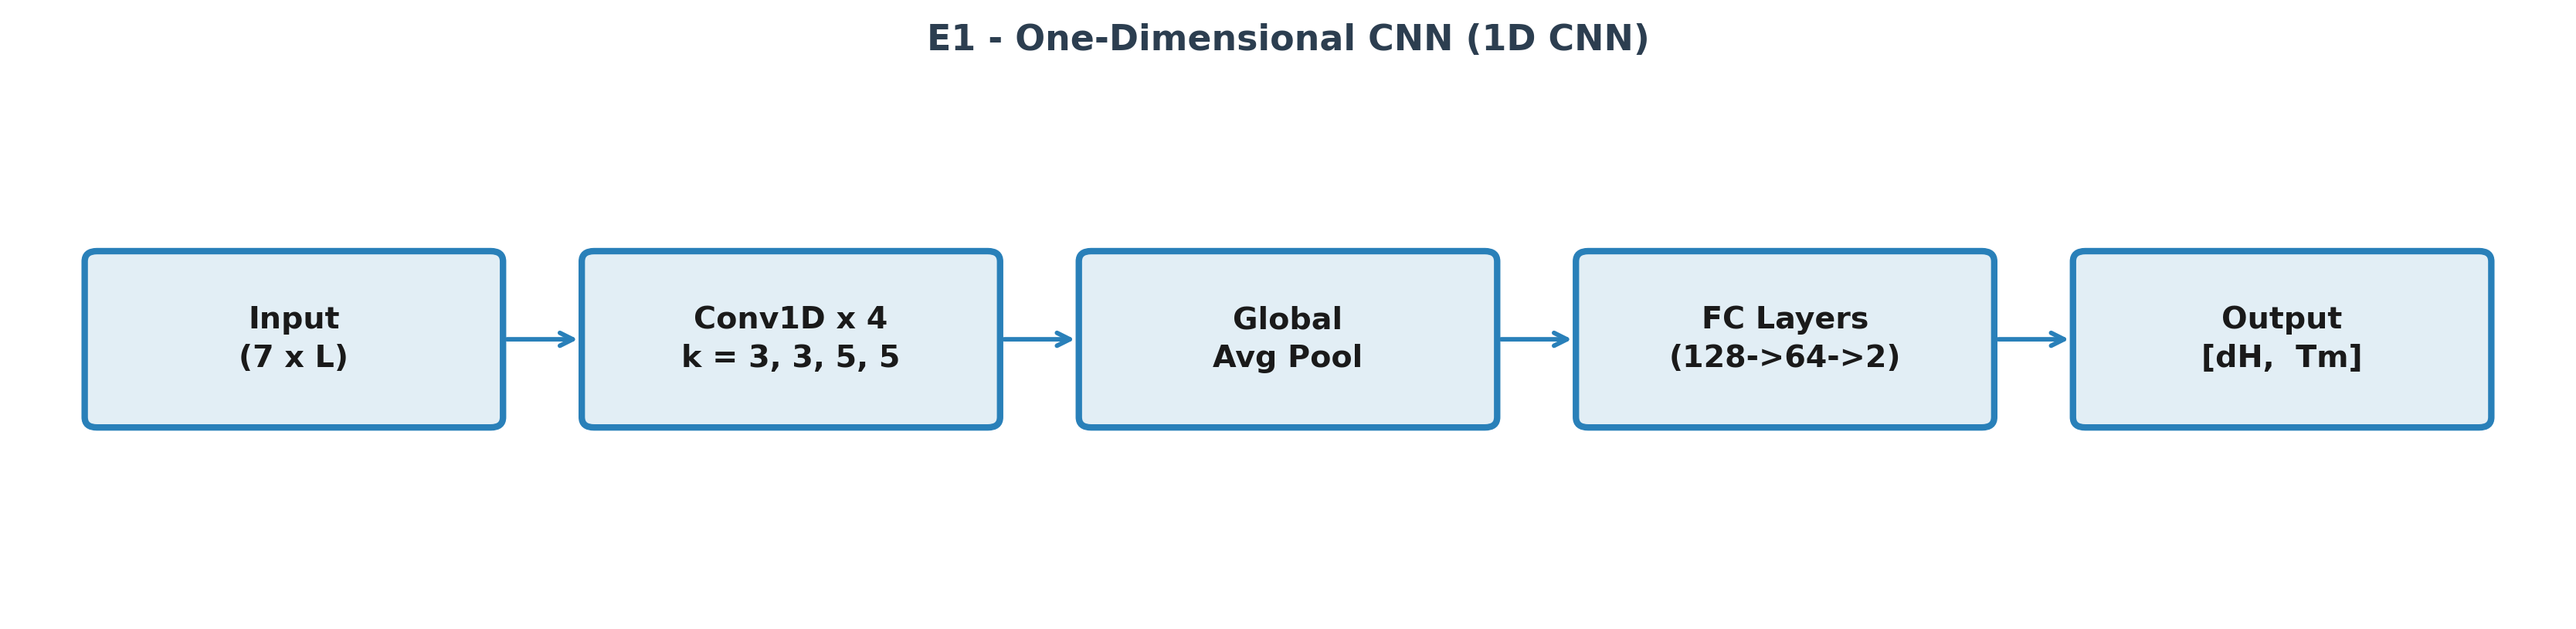
\includegraphics[width=\textwidth]{arch_e1_1dcnn.png}
    \caption{E1 --- One-Dimensional CNN (1D CNN). The sequence and secondary structure are encoded as a $7 \times L$ matrix ($L = 24$, zero-padded). Four Conv1D blocks with kernel sizes 3, 3, 5, 5 extract local motifs, followed by global average pooling and a 2-layer MLP predicting $[\hat{\Delta H}, \hat{T}_m]$.}
    \label{fig:arch_1dcnn}
\end{figure}

The 1D CNN encodes each sequence as a matrix of shape $(7 \times L)$ where $L = 24$ is the maximum sequence length and 7 is the number of input channels: 4 one-hot nucleotide channels plus 3 one-hot secondary structure channels (one each for \texttt{(}, \texttt{)}, \texttt{.}). Sequences shorter than 24 are zero-padded at the end.

The architecture applies four convolutional blocks in sequence:
\[
\text{Conv1d}(7, 64, k=3) \to \text{Conv1d}(64, 128, k=3) \to \text{Conv1d}(128, 128, k=5) \to \text{Conv1d}(128, 128, k=5)
\]
Each block includes BatchNorm, ReLU activation, and dropout. Global average pooling collapses the spatial dimension, and a 2-layer MLP produces the output.

\subsection{E2: Two-Dimensional Folded Ladder CNN (2D CNN)}

\begin{figure}[H]
    \centering
    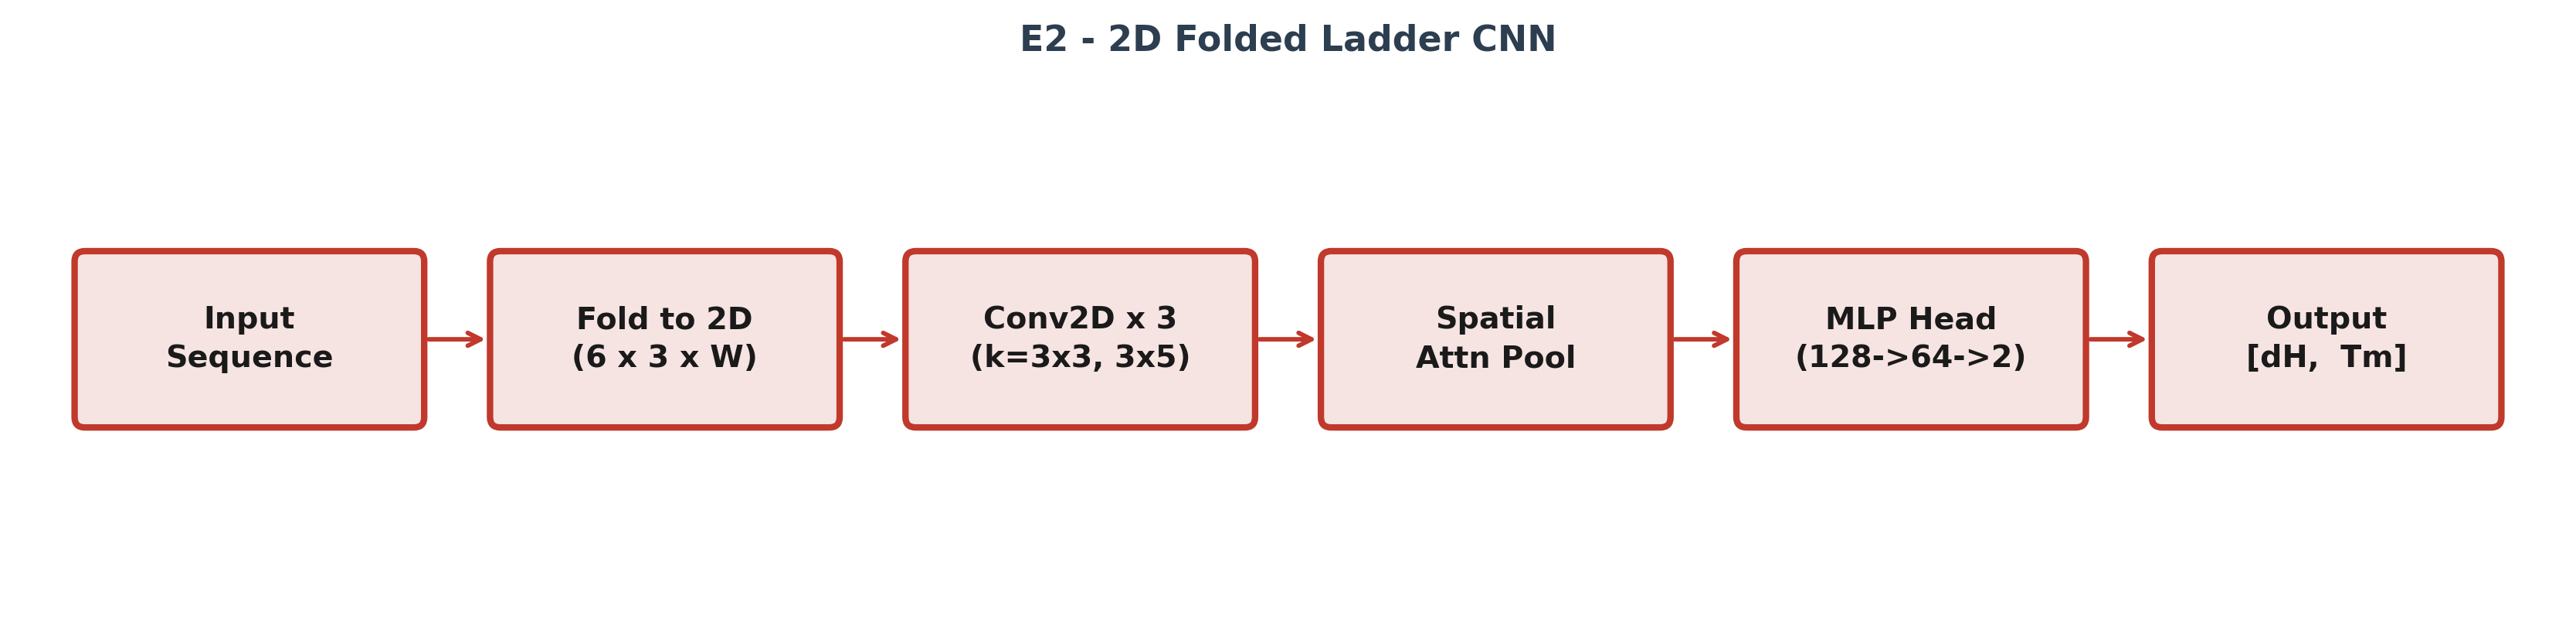
\includegraphics[width=\textwidth]{arch_e2_2dcnn.png}
    \caption{E2 --- Two-Dimensional Folded Ladder CNN (2D CNN). The hairpin is folded at its loop midpoint into a $6 \times 3 \times W$ tensor, aligning complementary bases in adjacent rows. Three Conv2D blocks extract spatial features, followed by learned attention pooling and a 2-layer MLP predicting $[\hat{\Delta H}, \hat{T}_m]$.}
    \label{fig:arch_2dcnn}
\end{figure}

The 2D Folded Ladder encoding is the principal novel contribution of this thesis. A DNA hairpin with $s$ stem pairs and $\ell$ loop nucleotides is folded computationally as follows:

\begin{enumerate}
    \item The fold point is defined at the loop midpoint: the first $s + \lfloor \ell/2 \rfloor$ nucleotides form the top strand (5$'$ arm + left half of loop).
    \item The remaining nucleotides form the bottom strand, reversed so that paired bases align in the same column.
    \item A middle row encodes the hydrogen bond pattern: 1 for stem positions, 0 for loop positions.
    \item A backbone turn column marks the fold point.
\end{enumerate}

The resulting tensor has shape $(6 \times 3 \times W)$ where $W = 15$ is the maximum width, and the 6 channels encode: one-hot nucleotide identity (4 channels), hydrogen bond indicator (1 channel), and backbone turn marker (1 channel).

\begin{figure}[h!]
    \centering
    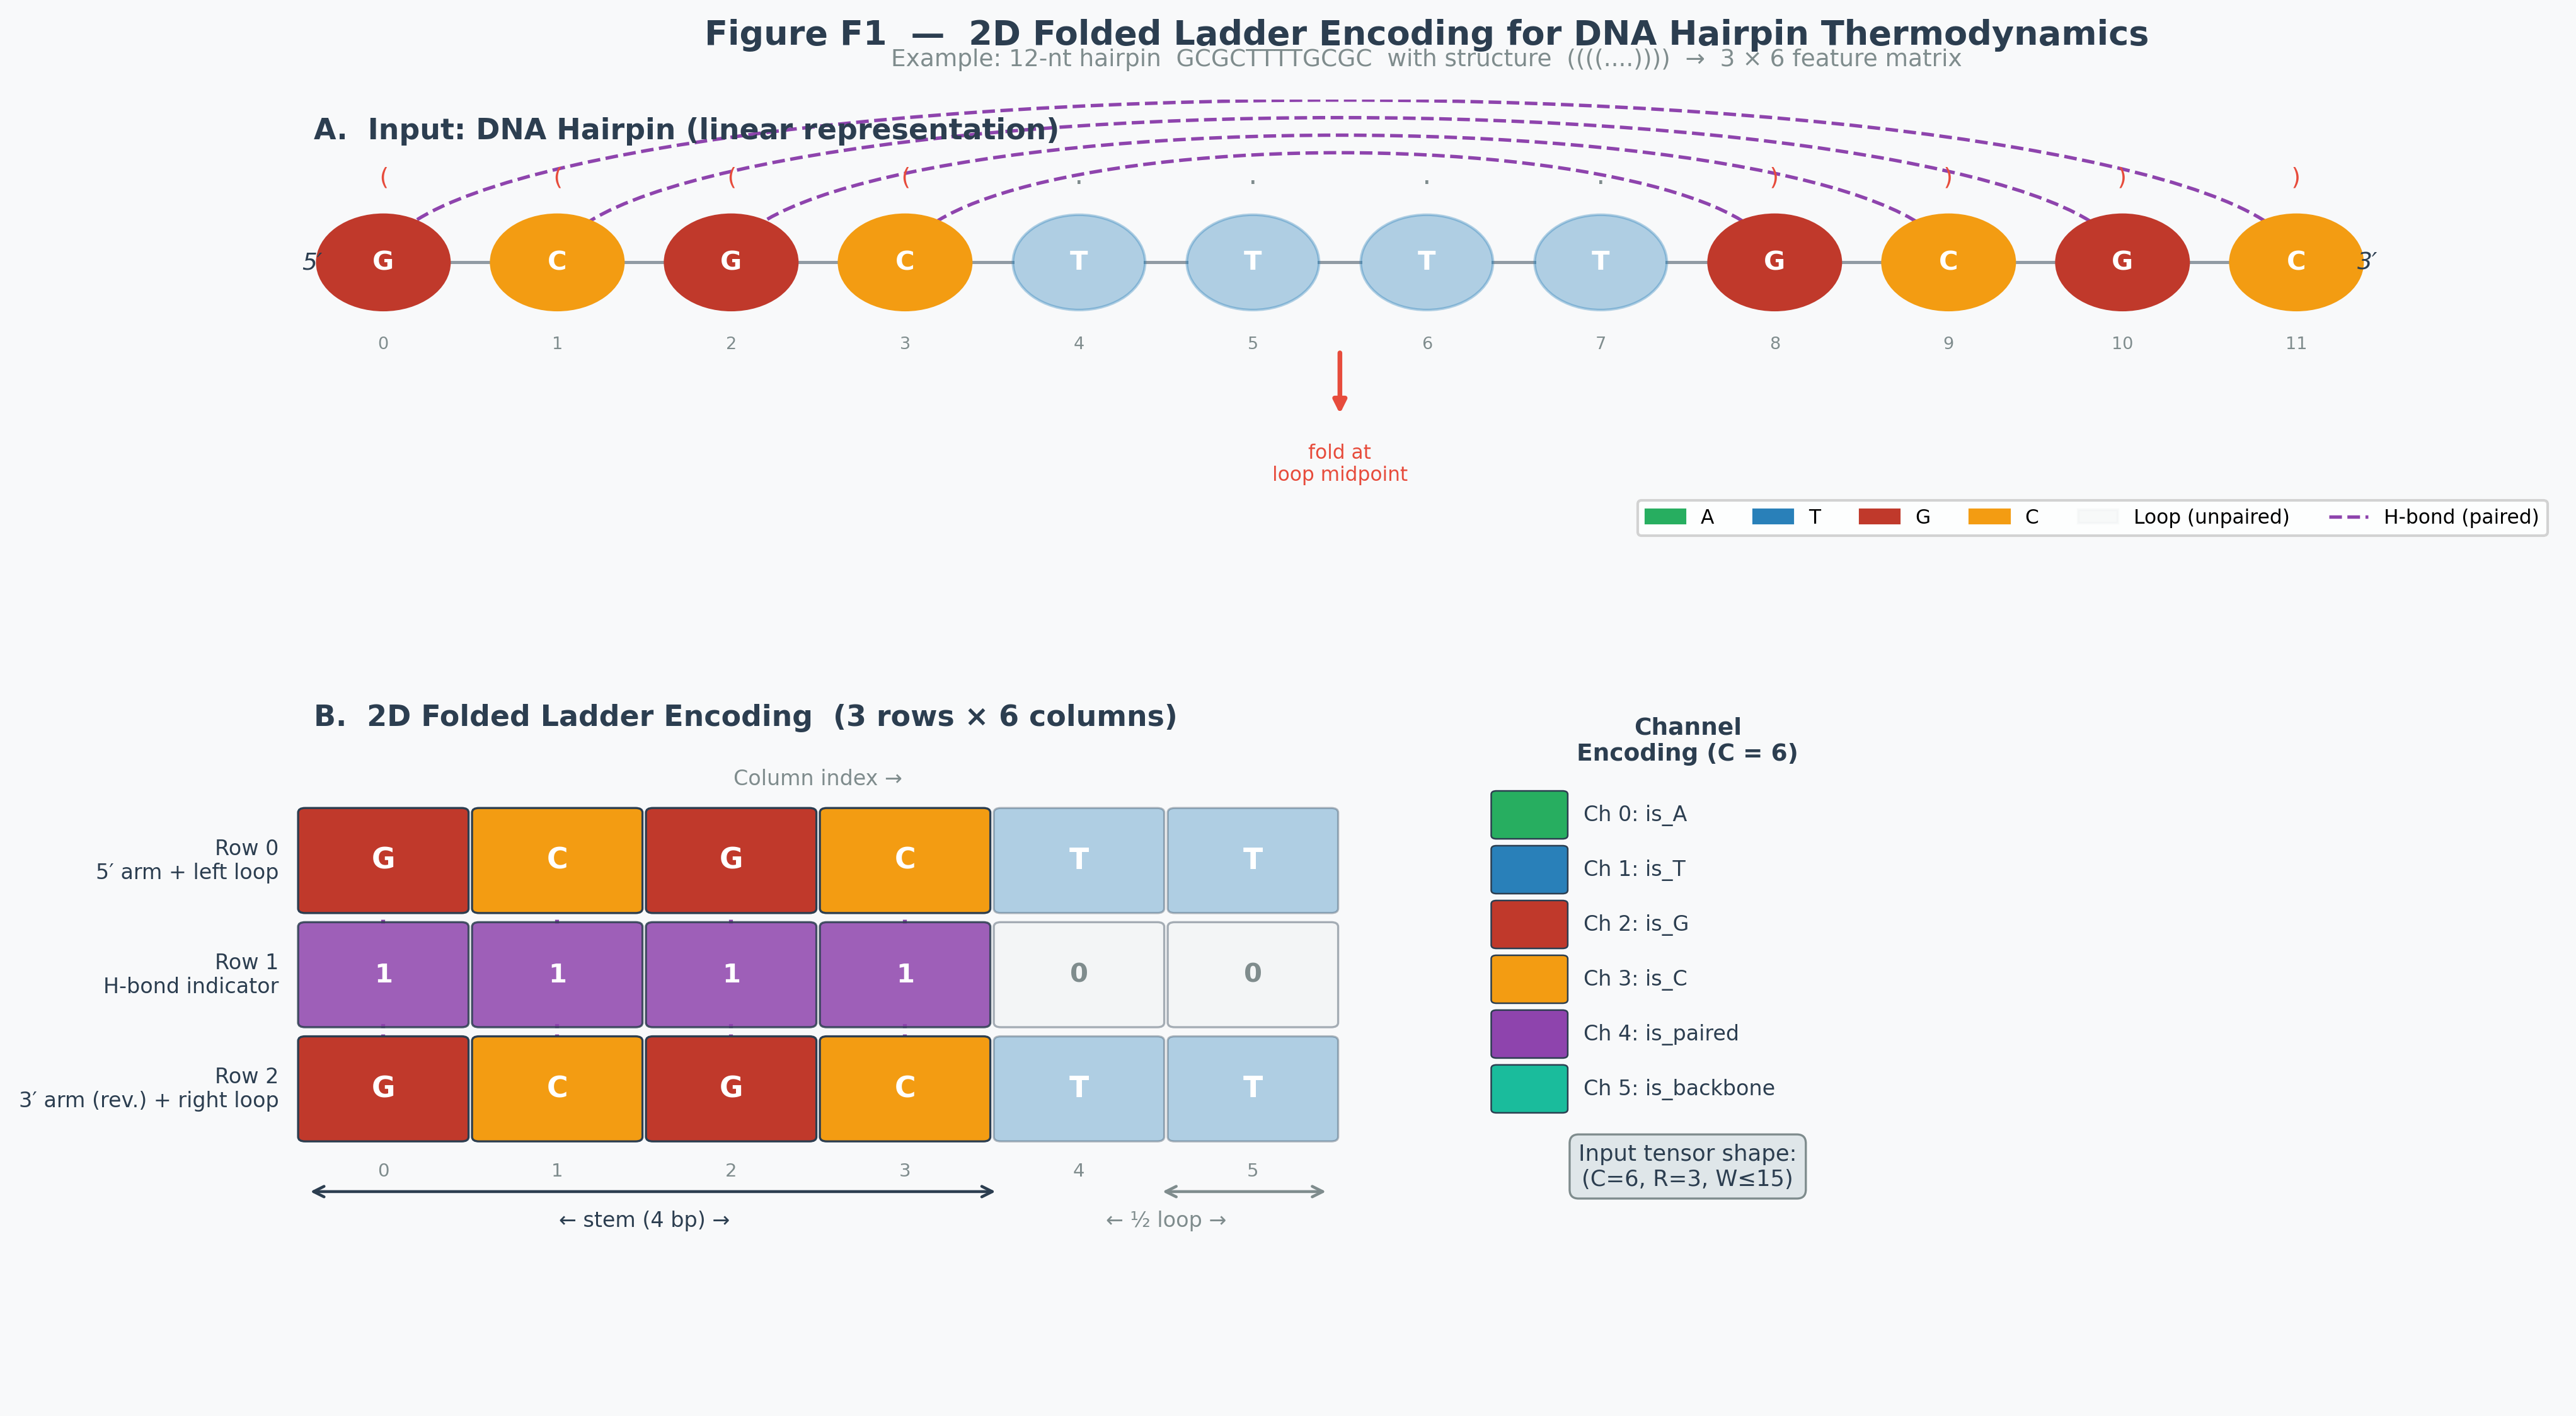
\includegraphics[width=0.85\textwidth]{folded_ladder_diagram.png}
    \caption{The 2D Folded Ladder encoding. A DNA hairpin (top) is folded at the loop midpoint to produce a three-row matrix (bottom) where base-paired nucleotides are aligned in the same column. The middle row encodes hydrogen bond presence. This spatial alignment means that a $3 \times k$ 2D convolutional filter with $k \geq 2$ directly captures a stack of $k$ adjacent base pairs, including the hydrogen bond between them.}
    \label{fig:folded_ladder}
\end{figure}

The model architecture applies three 2D convolutional blocks:
\[
\text{Conv2d}(6, 64, 3{\times}3) \to \text{Conv2d}(64, 128, 3{\times}3) \to \text{Conv2d}(128, 128, 3{\times}5)
\]
followed by learned attention pooling and a 2-layer MLP head. The spatial attention pooling learns per-position importance weights over the 2D feature map before global aggregation:

\begin{equation}
    \alpha_{ij} = \text{softmax}_{(i,j)}\left( \mathbf{v}^\top \tanh(\mathbf{W} \mathbf{h}_{ij}) \right)
    \label{eq:attn2d}
\end{equation}

\begin{equation}
    \mathbf{z} = \sum_{i,j} \alpha_{ij} \cdot \mathbf{h}_{ij}
    \label{eq:attnpool}
\end{equation}

where $\mathbf{h}_{ij}$ is the feature vector at spatial position $(i,j)$ and $\mathbf{z}$ is the pooled global representation.

\subsection{E3: Structure-Aware Transformer (SAT)}

\begin{figure}[H]
    \centering
    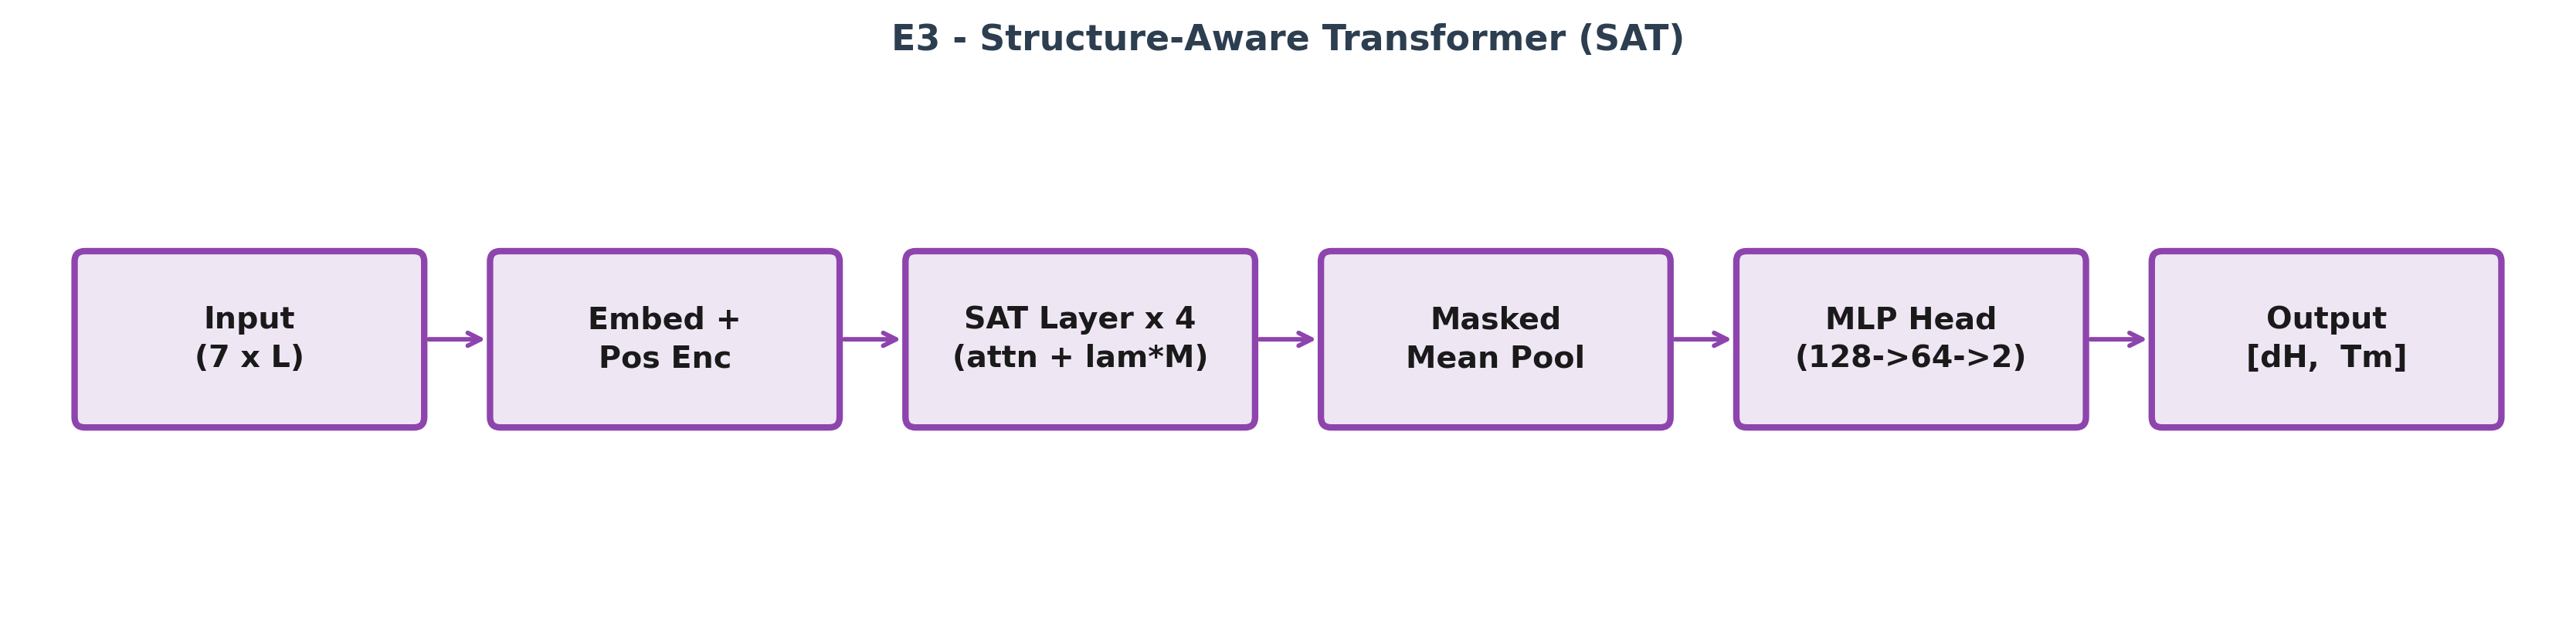
\includegraphics[width=\textwidth]{arch_e3_sat.png}
    \caption{E3 --- Structure-Aware Transformer (SAT). Token embeddings are augmented with positional encodings and passed through four SAT encoder layers. Each layer injects the structural adjacency matrix $M$ as an additive bias $\lambda M$ into the self-attention logits. Masked mean pooling and a 2-layer MLP produce $[\hat{\Delta H}, \hat{T}_m]$.}
    \label{fig:arch_sat}
\end{figure}

The Structure-Aware Transformer modifies the standard multi-head self-attention computation by injecting the structural adjacency matrix $M \in \{0,1\}^{L \times L}$ as an additive bias to the attention logits:

\begin{equation}
    \text{Attention}(Q, K, V) = \text{softmax}\left( \frac{QK^\top}{\sqrt{d_\text{head}}} + \lambda M \right) V
    \label{eq:sat}
\end{equation}

where $\lambda$ is a learnable scalar parameter per layer that controls the influence of the structural prior. $M$ is a symmetric binary matrix where $M_{ij} = 1$ if nucleotides $i$ and $j$ are hydrogen-bonded (from dot-bracket) or backbone-adjacent ($|i-j|=1$), and 0 otherwise.

The intuition is that standard self-attention treats all position pairs equally at initialization; the structural bias $\lambda M$ explicitly tells the model which pairs are physically connected, guiding the attention distribution toward structurally relevant relationships. $\lambda$ is initialized to 1.0 and allowed to decay during training if the data does not support the structural bias.

The full architecture uses 4 SAT encoder layers with $d_{\text{model}} = 128$, 8 attention heads, and a feed-forward dimension of 256. Masked mean pooling over non-padding positions produces the sequence representation, followed by a 2-layer MLP head.

\subsection{E4: Physics-Informed Neural Network (PINN)}

\begin{figure}[H]
    \centering
    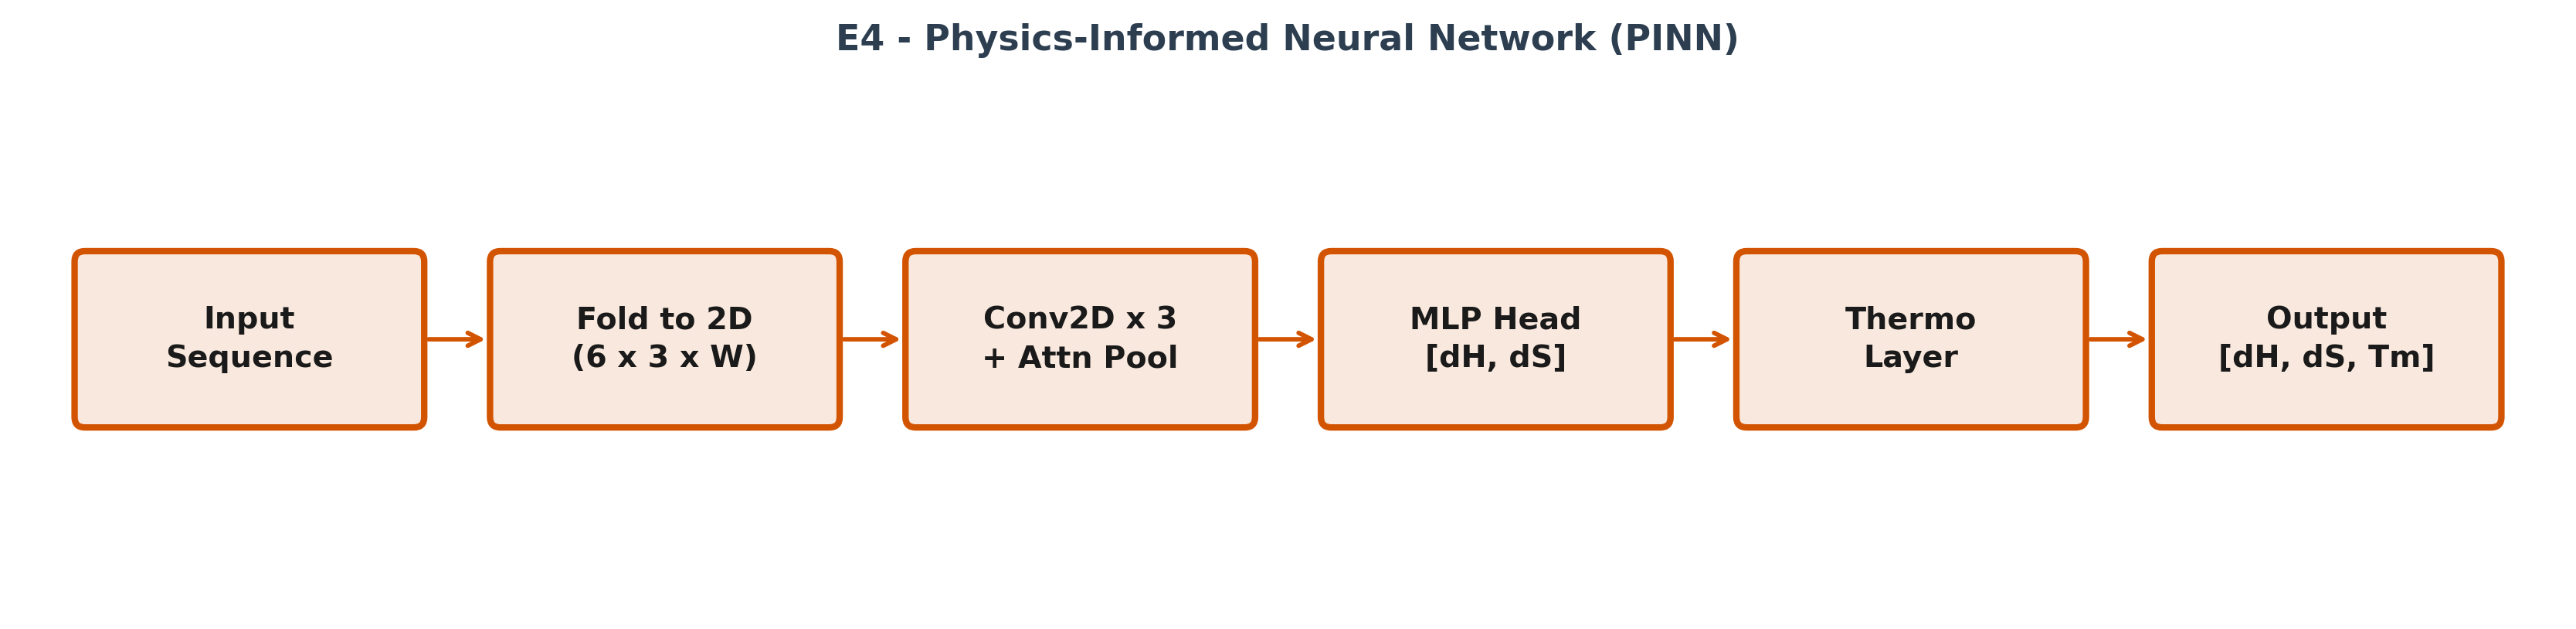
\includegraphics[width=\textwidth]{arch_e4_pinn.png}
    \caption{E4 --- Physics-Informed Neural Network (PINN). Shares the Conv2D backbone and attention pooling of E2. The MLP head predicts $[\hat{\Delta H}_{\text{norm}}, \hat{\Delta S}_{\text{norm}}]$ rather than $T_m$ directly. A fixed \texttt{ThermodynamicsLayer} derives $\hat{T}_m$ analytically via $T_m = \Delta H / \Delta S - 273.15$, and a physics penalty $\mathcal{P}$ enforces thermodynamic constraints during training.}
    \label{fig:arch_pinn}
\end{figure}

The PINN modifies the 2D CNN backbone (same architecture as E2) by changing what the output head predicts. Instead of predicting $[\hat{\Delta H}, \hat{T}_m]$ directly, the model predicts $[\hat{\Delta H}_{\text{norm}}, \hat{\Delta S}_{\text{norm}}]$, and then computes $\hat{T}_m$ inside the forward pass using the thermodynamic identity:

\begin{equation}
    \hat{T}_m = \frac{\hat{\Delta H}}{\hat{\Delta S}} - 273.15
    \label{eq:pinn_tm}
\end{equation}

where $\hat{\Delta H}$ and $\hat{\Delta S}$ are unnormalized from their respective prediction ranges. This \texttt{ThermodynamicsLayer} is not learnable; it applies Equation~\ref{eq:pinn_tm} exactly. The training loss combines supervised regression with a physical violation penalty:

\begin{equation}
    \mathcal{L} = \text{MSE}(\hat{\Delta H}_{\text{norm}}, {\Delta H}_{\text{norm}}^*) + \text{MSE}(\hat{T}_{m,\text{norm}}, T_{m,\text{norm}}^*) + \alpha \cdot \mathcal{P}
    \label{eq:pinn_loss}
\end{equation}

where $\alpha = 0.1$ and the physical penalty $\mathcal{P}$ penalizes thermodynamically impossible predictions:

\begin{equation}
    \mathcal{P} = \text{ReLU}(\hat{\Delta H}) + \text{ReLU}(\hat{\Delta S}) + \text{ReLU}(\hat{\Delta H} - 310.15 \cdot \hat{\Delta S})
    \label{eq:penalty}
\end{equation}

The three terms in $\mathcal{P}$ enforce that $\Delta H < 0$ (exothermic hybridization), $\Delta S < 0$ (unfavorable entropy of ordering), and $\Delta G_{37} < 0$ (spontaneous folding at 37$^\circ$C).

\subsection{E5: Hybrid CNN-RNN}

\begin{figure}[H]
    \centering
    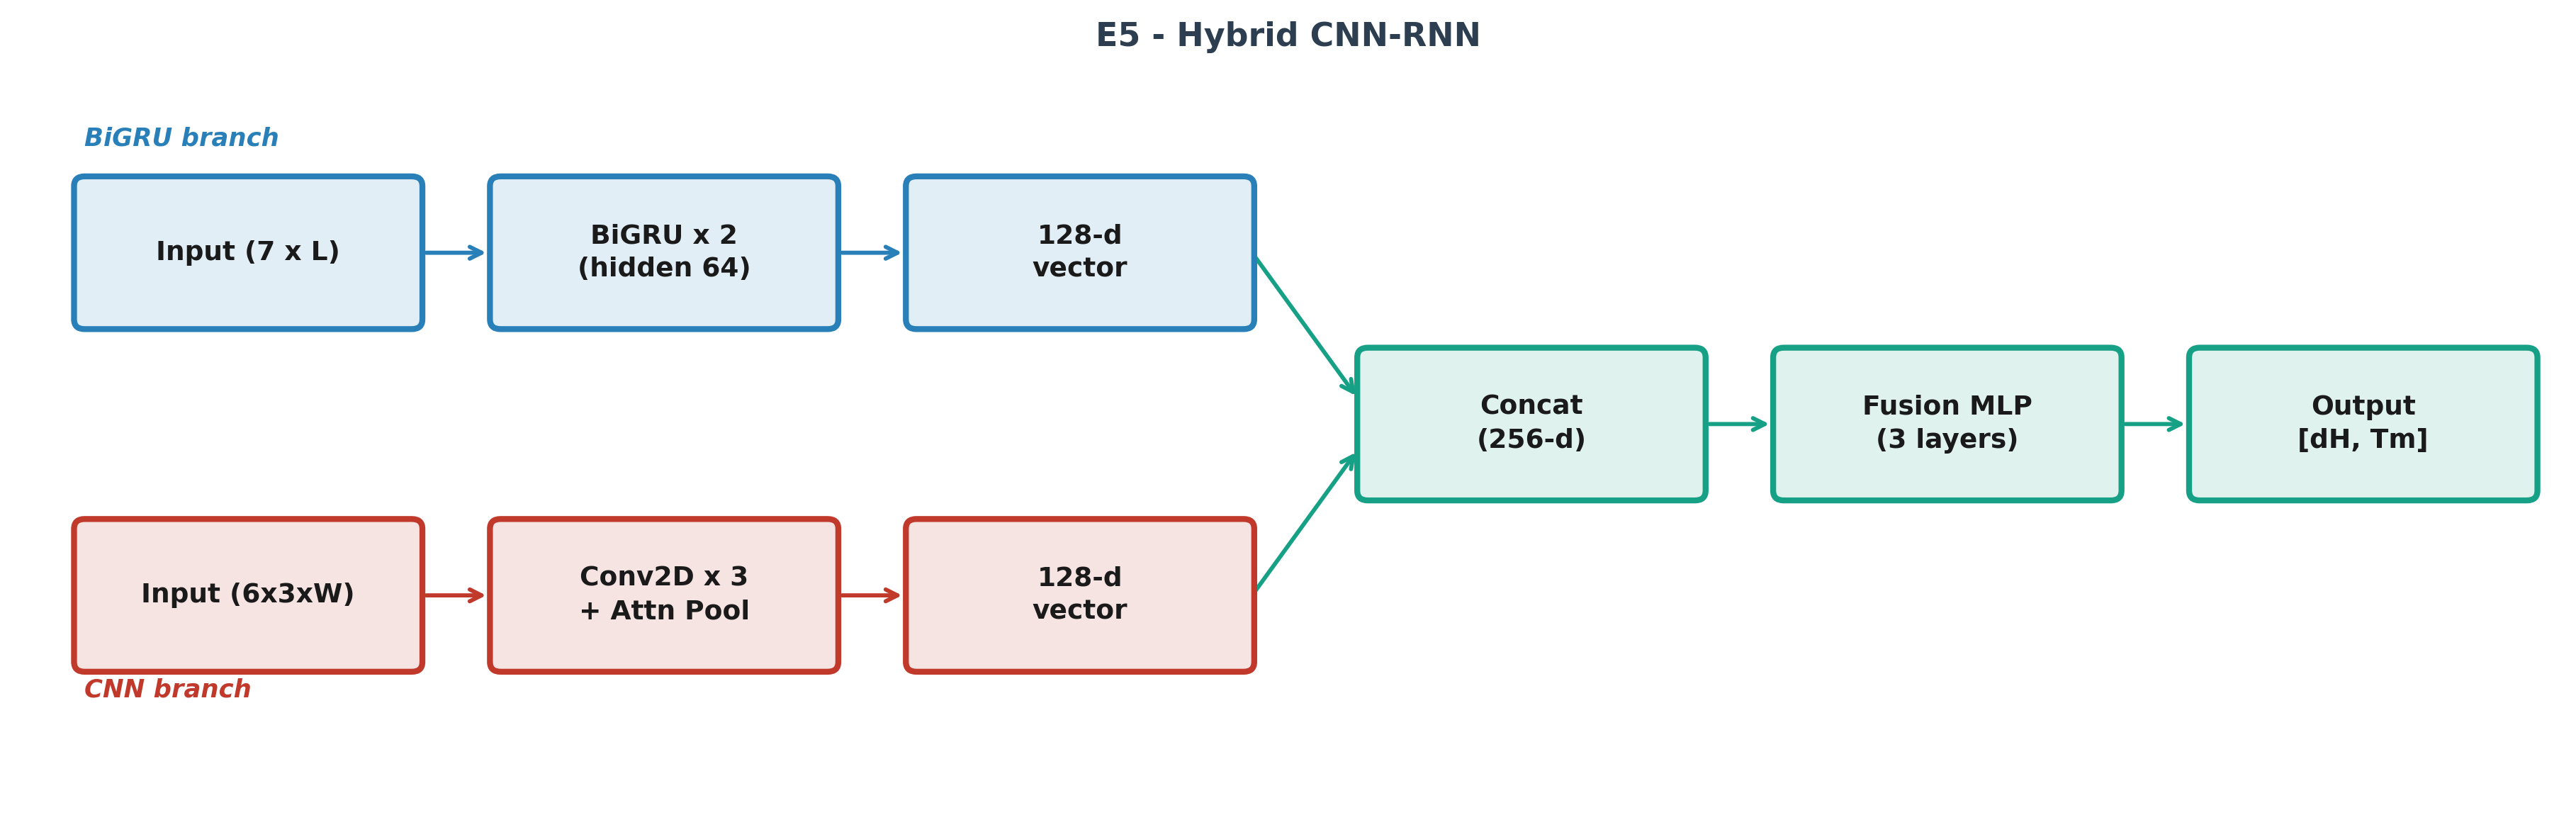
\includegraphics[width=\textwidth]{arch_e5_hybrid.png}
    \caption{E5 --- Hybrid CNN-RNN. Two parallel branches process the input: a BiGRU branch (blue) encodes sequential unzipping dynamics; a 2D CNN branch (red) captures spatial base-pairing geometry. Their 128-dimensional outputs are concatenated to form a 256-dimensional representation, which a 3-layer fusion MLP maps to $[\hat{\Delta H}, \hat{T}_m]$.}
    \label{fig:arch_hybrid}
\end{figure}

The Hybrid model processes the input through two parallel branches and concatenates their latent representations:

\begin{enumerate}
    \item \textbf{BiGRU branch}: takes the sequence as a $(L \times 7)$ time-series input (same encoding as the 1D CNN) and processes it through a 2-layer bidirectional GRU with hidden size 64. Masked mean pooling over non-padding positions produces a 128-dimensional vector.
    \item \textbf{2D CNN branch}: takes the folded ladder tensor $(6 \times 3 \times W)$ and processes it through the same three convolutional blocks as E2, followed by attention pooling, producing a 128-dimensional vector.
\end{enumerate}

The two 128-dimensional vectors are concatenated to form a 256-dimensional representation, which is passed through a 3-layer fusion MLP with hidden dimensions 128 and 64, producing the output $[\hat{\Delta H}_{\text{norm}}, \hat{T}_{m,\text{norm}}]$.

\section{Training Protocol}

All six models use the same training protocol to ensure fair comparison:

\begin{itemize}
    \item \textbf{Optimizer}: Adam~\cite{kingma2015} with learning rate $10^{-3}$ and weight decay $10^{-5}$.
    \item \textbf{Learning rate schedule}: Cosine annealing from $10^{-3}$ to $10^{-5}$ over 200 epochs.
    \item \textbf{Loss}: Mean squared error on normalized $[\hat{\Delta H}, \hat{T}_m]$ (or as modified for E4).
    \item \textbf{Gradient clipping}: maximum norm 1.0.
    \item \textbf{Batch size}: 256 sequences.
    \item \textbf{Training set}: \texttt{arr} partition only (25,009 sequences after NaN removal).
    \item \textbf{Model selection}: best checkpoint selected by minimum $\Delta G_{37}$ MAE on the validation set.
    \item \textbf{WandB logging}: all runs logged to the \texttt{NNN\_Thesis\_Experiments} project.
\end{itemize}

All experiments were run on a single NVIDIA GPU using PyTorch 1.x and PyTorch Geometric.

\section{Evaluation Metrics}

For each model and each target quantity $y \in \{\Delta H, T_m, \Delta G_{37}\}$, I compute:

\begin{itemize}
    \item Mean Absolute Error: $\text{MAE} = \frac{1}{n}\sum_{i=1}^n |y_i - \hat{y}_i|$
    \item Root Mean Square Error: $\text{RMSE} = \sqrt{\frac{1}{n}\sum_{i=1}^n (y_i - \hat{y}_i)^2}$
    \item Coefficient of determination: $R^2 = 1 - \frac{\sum(y_i - \hat{y}_i)^2}{\sum(y_i - \bar{y})^2}$
\end{itemize}

For the out-of-distribution evaluation on \texttt{lit\_uv}, only $T_m$ MAE is reported because the \texttt{lit\_uv} sequences do not have measured $\Delta H$ values.

\section{The SantaLucia Classical Baseline}

As an additional reference point, I implement the SantaLucia 2004 nearest-neighbor model~\cite{santalucia2004} from scratch using the published $\Delta H$ and $\Delta S$ parameters for all 10 Watson-Crick dinucleotide stacks, initiation corrections for terminal base pairs, and the Owczarzy et al.~\cite{owczarzy2004} sodium correction formula:

\begin{equation}
    \frac{1}{T_m(\text{Na}^+)} = \frac{1}{T_m(1\,\text{M})} + (4.29 f_{GC} - 3.95) \times 10^{-5} \ln[\text{Na}^+] + 9.40 \times 10^{-6} (\ln[\text{Na}^+])^2
    \label{eq:owczarzy}
\end{equation}

where $f_{GC}$ is the fraction of G--C base pairs in the duplex. The sodium concentration and DNA concentration for each \texttt{lit\_uv} sequence are taken from the dataset's \texttt{sodium} and \texttt{DNA\_conc} columns. This baseline uses no learned parameters and is evaluated on the same 348 sequences as the neural network models.

% =========================================================
\chapter{Results}
% =========================================================

\section{In-Distribution Performance}

Table~\ref{tab:results_main} summarizes the validation performance of all six models on the \texttt{arr} held-out validation set.

\begin{table}[h!]
\centering
\caption{Validation set performance on the \texttt{arr} dataset. All models trained on \texttt{arr} training sequences only. $\Delta G_{37}$ is derived, not directly predicted.}
\label{tab:results_main}
\begin{tabular}{llrrrrrr}
\toprule
ID & Model & $\Delta H$ MAE & $T_m$ MAE & $\Delta G_{37}$ MAE & $T_m$ RMSE & $T_m$ $R^2$ \\
   &       & (kcal/mol) & ($^\circ$C) & (kcal/mol) & ($^\circ$C) & \\
\midrule
E0 & GNN   & 3.682 & 3.283 & 0.266 & 4.311 & 0.840 \\
E1 & 1D CNN & 2.911 & 1.808 & 0.177 & 2.556 & 0.947 \\
E3 & SAT   & 3.419 & 2.251 & 0.217 & 3.063 & 0.908 \\
E4 & PINN  & 3.597 & 2.754 & 0.195 & 3.841 & 0.866 \\
E2 & 2D CNN & 2.846 & 1.568 & 0.156 & 2.345 & 0.957 \\
E5 & Hybrid & \textbf{2.814} & \textbf{1.530} & \textbf{0.155} & \textbf{2.267} & \textbf{0.959} \\
\bottomrule
\end{tabular}
\end{table}

The Hybrid CNN-RNN (E5) achieves the best performance on all metrics, with $T_m$ MAE of 1.53$^\circ$C and $R^2 = 0.959$. The 2D CNN (E2) is a close second, with $T_m$ MAE of 1.57$^\circ$C. These two models substantially outperform the GNN baseline (E0), which achieves $T_m$ MAE of 3.28$^\circ$C --- a factor of more than two worse.

The 1D CNN (E1) performs considerably better than the GNN despite its simpler architecture, suggesting that the translation-invariant sequential bias is better suited to this dataset than the permutation-equivariant graph bias. The Structure-Aware Transformer (E3) and PINN (E4) occupy the middle of the performance range; both incorporate additional structure-related information but pay for it in optimization difficulty.

\section{Convergence Analysis}

Figure~\ref{fig:convergence} shows the validation $T_m$ MAE convergence curves for all six models over 200 training epochs.

\begin{figure}[h!]
    \centering
    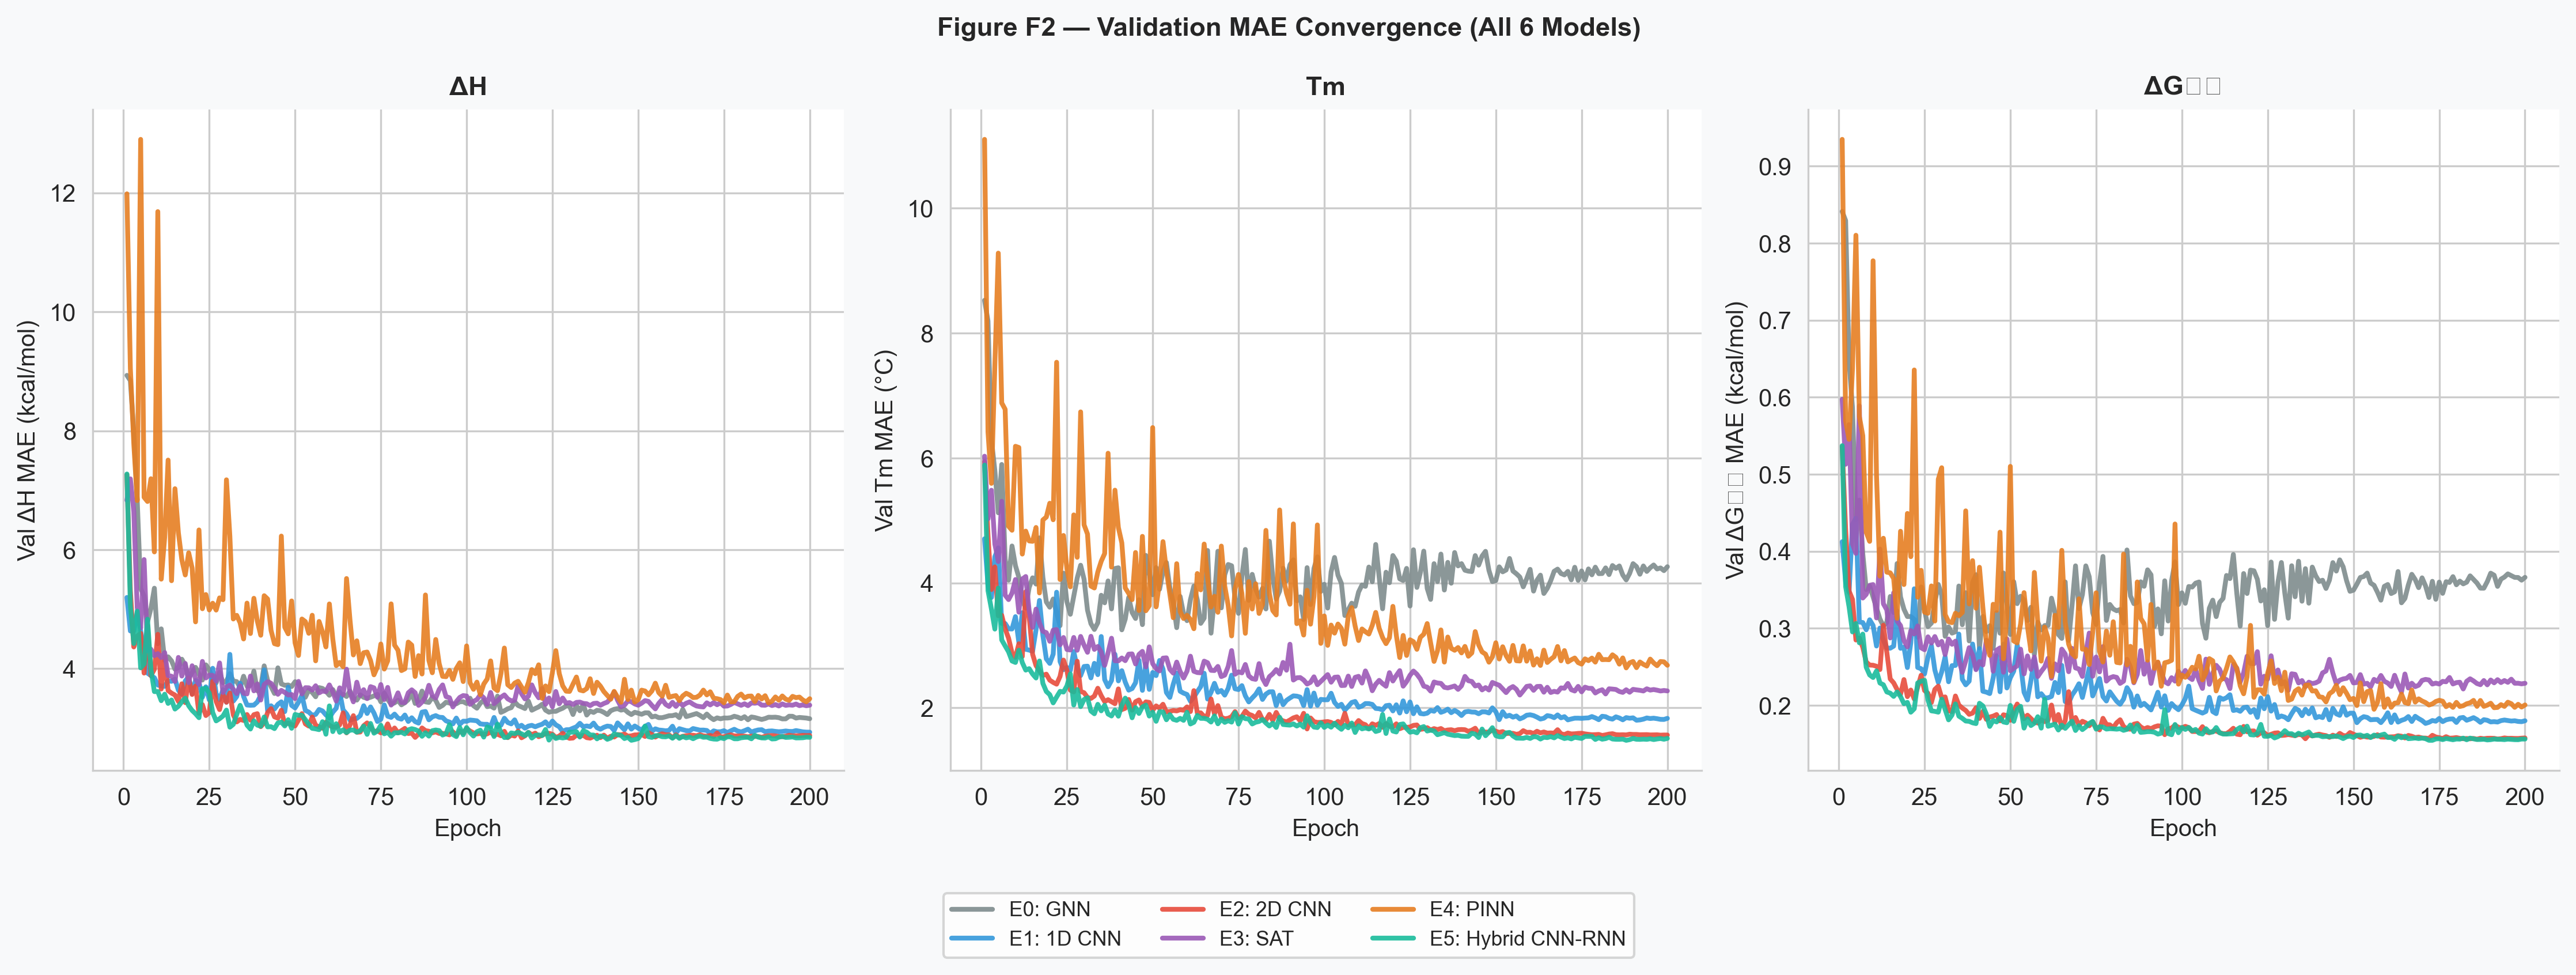
\includegraphics[width=\textwidth]{convergence_curves.png}
    \caption{Validation MAE convergence over 200 training epochs for all six models. All three targets ($\Delta H$, $T_m$, $\Delta G_{37}$) are shown. E5 (Hybrid) and E2 (2D CNN) converge fastest and to the lowest error. The GNN (E0) shows slow convergence, consistent with the known optimization challenges of graph neural networks on this type of data.}
    \label{fig:convergence}
\end{figure}

A few observations stand out. First, the GNN (E0) converges more slowly than all other models and reaches a substantially higher final error. This is consistent with findings in the molecular property prediction literature that GNN training is more sensitive to the initialization and learning rate schedule than convolutional models. Second, the PINN (E4) shows noticeably noisier training dynamics compared to the other 2D CNN-based models; the physics penalty introduces gradient conflicts that make optimization less smooth. Third, the Hybrid model (E5) converges consistently and reaches the lowest final error, suggesting that the dual-modality input provides complementary gradient signals.

\section{Predicted vs.\ Measured Scatter Analysis}

Figures~\ref{fig:scatter_a} and~\ref{fig:scatter_b} show the predicted versus measured scatter plots for all six models on the validation set, split into two groups for clarity.

\begin{figure}[h!]
    \centering
    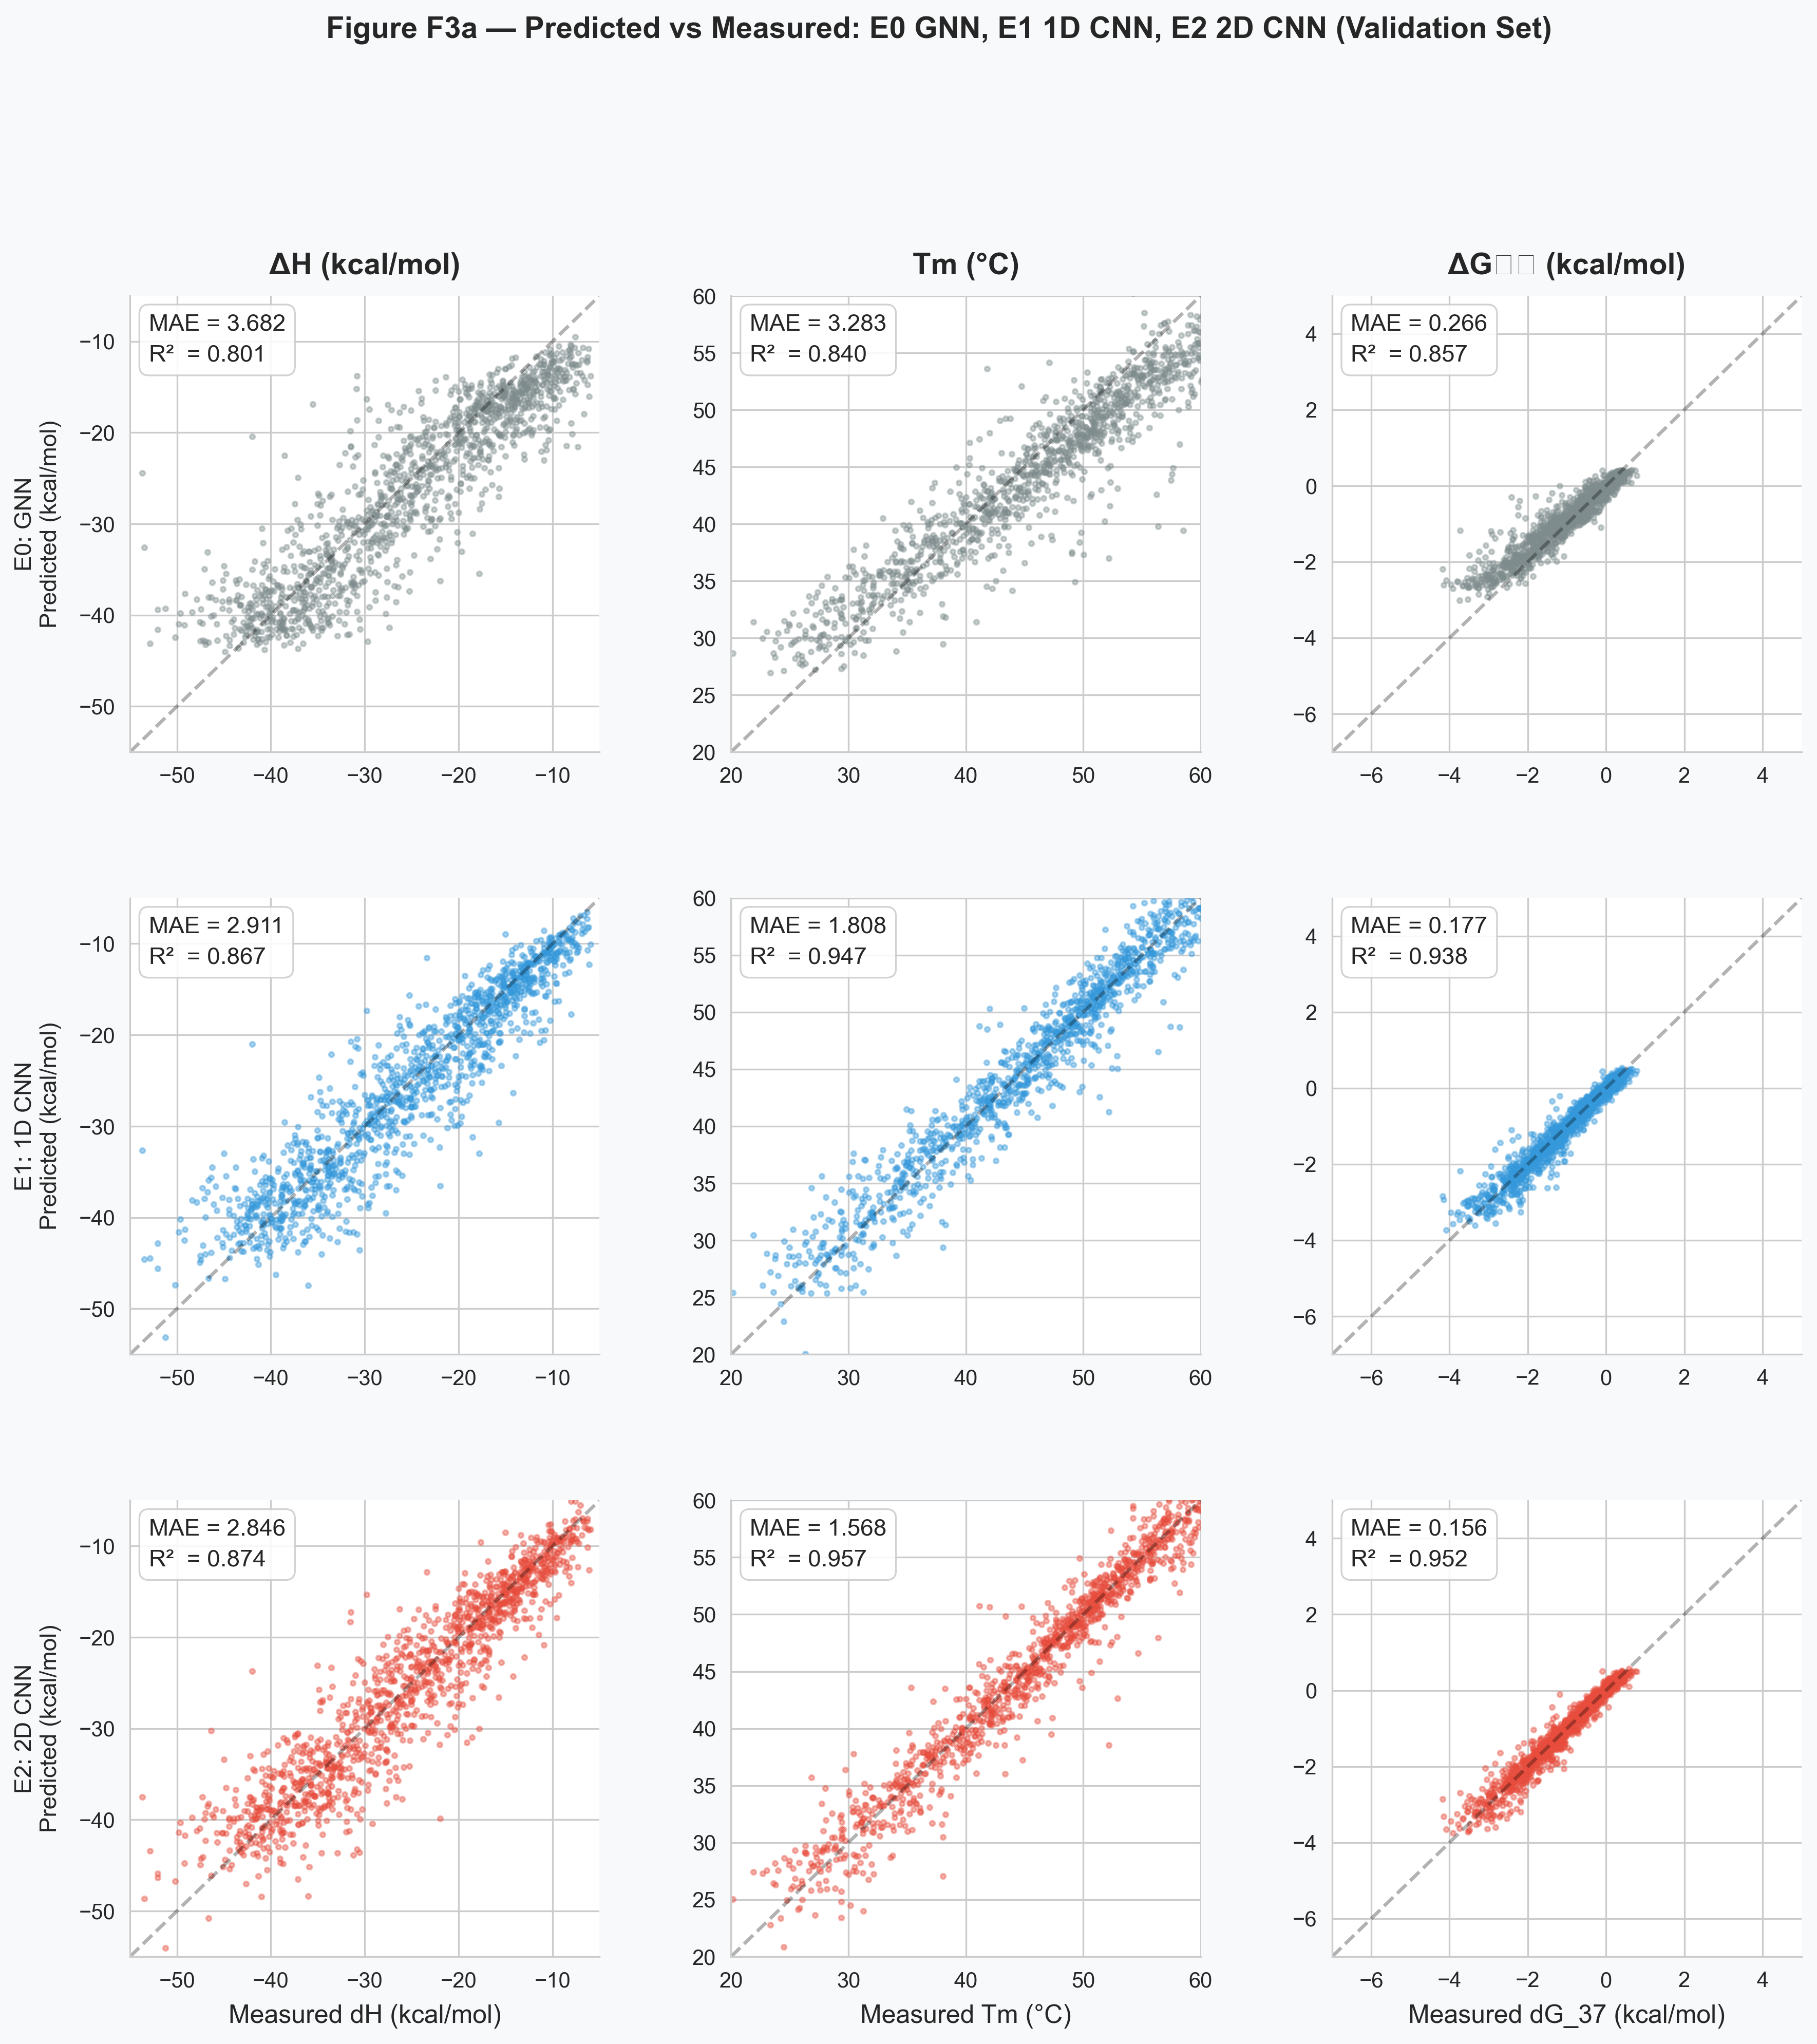
\includegraphics[width=\textwidth,keepaspectratio]{scatter_grid_a.png}
    \caption{Predicted versus measured values for $\Delta H$, $T_m$, and $\Delta G_{37}$ on the \texttt{arr} validation set for E0 (GNN), E1 (1D CNN), and E2 (2D CNN). Rows correspond to models; columns to target quantities. The dashed diagonal represents perfect prediction. The GNN (E0) shows notably wider scatter, particularly for $\Delta H$, while the 2D CNN (E2) achieves a tight, well-calibrated distribution across all three targets.}
    \label{fig:scatter_a}
\end{figure}

\begin{figure}[h!]
    \centering
    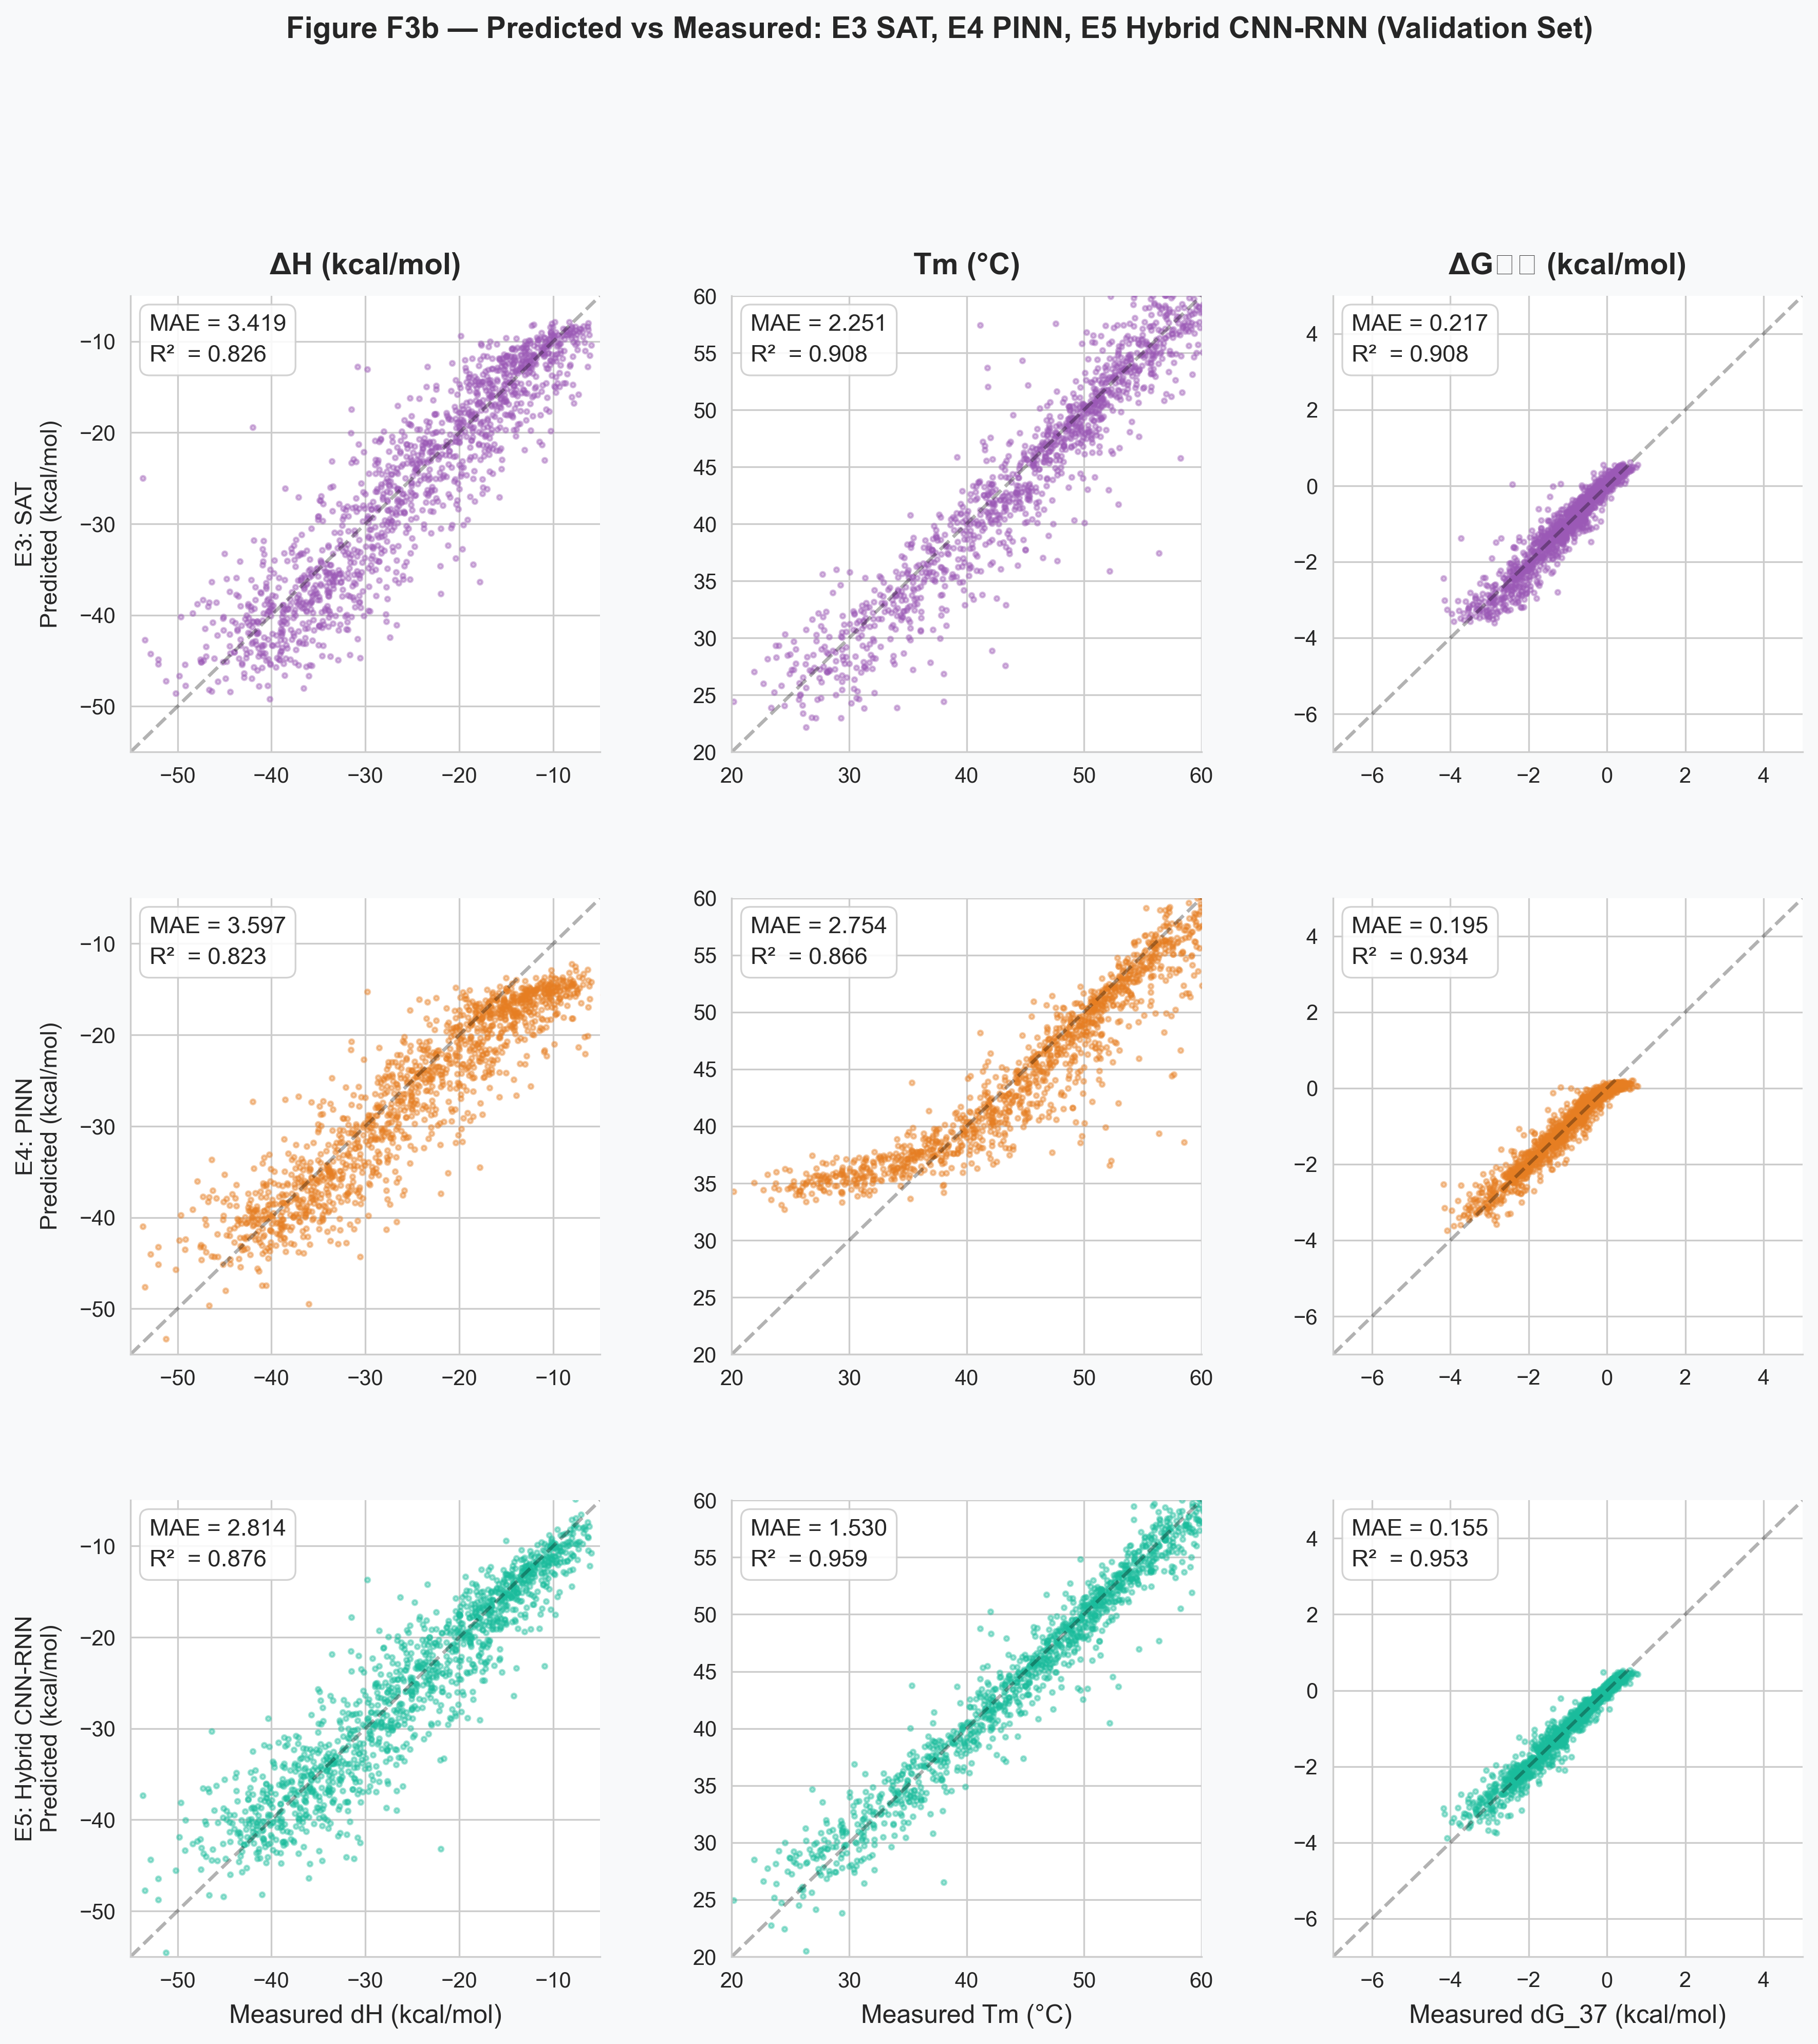
\includegraphics[width=\textwidth,keepaspectratio]{scatter_grid_b.png}
    \caption{Predicted versus measured values for $\Delta H$, $T_m$, and $\Delta G_{37}$ on the \texttt{arr} validation set for E3 (SAT), E4 (PINN), and E5 (Hybrid CNN-RNN). The Hybrid (E5) and SAT (E3) models achieve tight clustering around the diagonal for $T_m$; the PINN (E4) shows slightly wider $\Delta H$ scatter consistent with its noisier training dynamics.}
    \label{fig:scatter_b}
\end{figure}

The scatter plots confirm the ranking in Table~\ref{tab:results_main}. The GNN scatter (E0) is notably wider, particularly for $\Delta H$, where the model systematically underpredicts the magnitude of enthalpy for strongly negative sequences. The 2D CNN (E2) and Hybrid (E5) models show well-calibrated predictions across the full range of values for all three targets.

\section{Model Complexity}

Table~\ref{tab:params} reports the number of trainable parameters for each model. The 1D CNN and 2D CNN have the fewest parameters while achieving competitive or superior performance, which is a positive indicator of data efficiency. The GNN has a moderate parameter count but the highest validation error, suggesting that its inductive bias is a poorer fit for this task.

\begin{table}[h!]
\centering
\caption{Trainable parameter counts for all six models.}
\label{tab:params}
\begin{tabular}{llr}
\toprule
ID & Model & Parameters \\
\midrule
E0 & GNN   & $\sim$252,000 \\
E1 & 1D CNN & $\sim$156,000 \\
E2 & 2D CNN & $\sim$198,000 \\
E3 & SAT   & $\sim$412,000 \\
E4 & PINN  & $\sim$200,000 \\
E5 & Hybrid & $\sim$326,000 \\
\bottomrule
\end{tabular}
\end{table}

% =========================================================
\chapter{Generalization and Discussion}
% =========================================================

\section{Out-of-Distribution Generalization Results}

Table~\ref{tab:ood} and Figure~\ref{fig:ood} show the $T_m$ MAE on two external out-of-distribution evaluation sets: the \texttt{lit\_uv} literature UV melting dataset (348 perfectly complementary Watson-Crick duplexes) and the \texttt{ov} Oliveira et al.\ dataset (2,775 duplex sequences, 97.8\% of which contain at least one internal mismatch or bulge~\cite{oliveira2020}). All models were trained exclusively on \texttt{arr} hairpin sequences and evaluated without any fine-tuning.

\begin{table}[h!]
\centering
\caption{Out-of-distribution $T_m$ MAE ($^\circ$C) on two external duplex datasets. \texttt{lit\_uv}: 348 perfectly complementary Watson-Crick duplex sequences with varying ionic conditions. \texttt{ov}: 2,775 duplex sequences from Oliveira et al.~\cite{oliveira2020} of which 97.8\% contain at least one internal mismatch or bulge. The SantaLucia model uses no learned parameters; its \texttt{ov} performance reflects the absence of mismatch-specific parameters. Bold values indicate the best deep learning model for each dataset.}
\label{tab:ood}
\begin{tabular}{llrr}
\toprule
ID & Model & lit\_uv $T_m$ MAE ($^\circ$C) & ov $T_m$ MAE ($^\circ$C) \\
\midrule
NN & SantaLucia (2004) & \textbf{1.852} & 9.938 \\
\midrule
E0 & GNN     & \textbf{5.590} & \textbf{5.273} \\
E4 & PINN    & 5.857          & 11.776 \\
E1 & 1D CNN  & 6.316          & 20.461 \\
E3 & SAT     & 8.597          & 9.246 \\
E5 & Hybrid  & 8.265          & 21.059 \\
E2 & 2D CNN  & 9.945          & 12.836 \\
\bottomrule
\end{tabular}
\end{table}

\begin{figure}[h!]
    \centering
    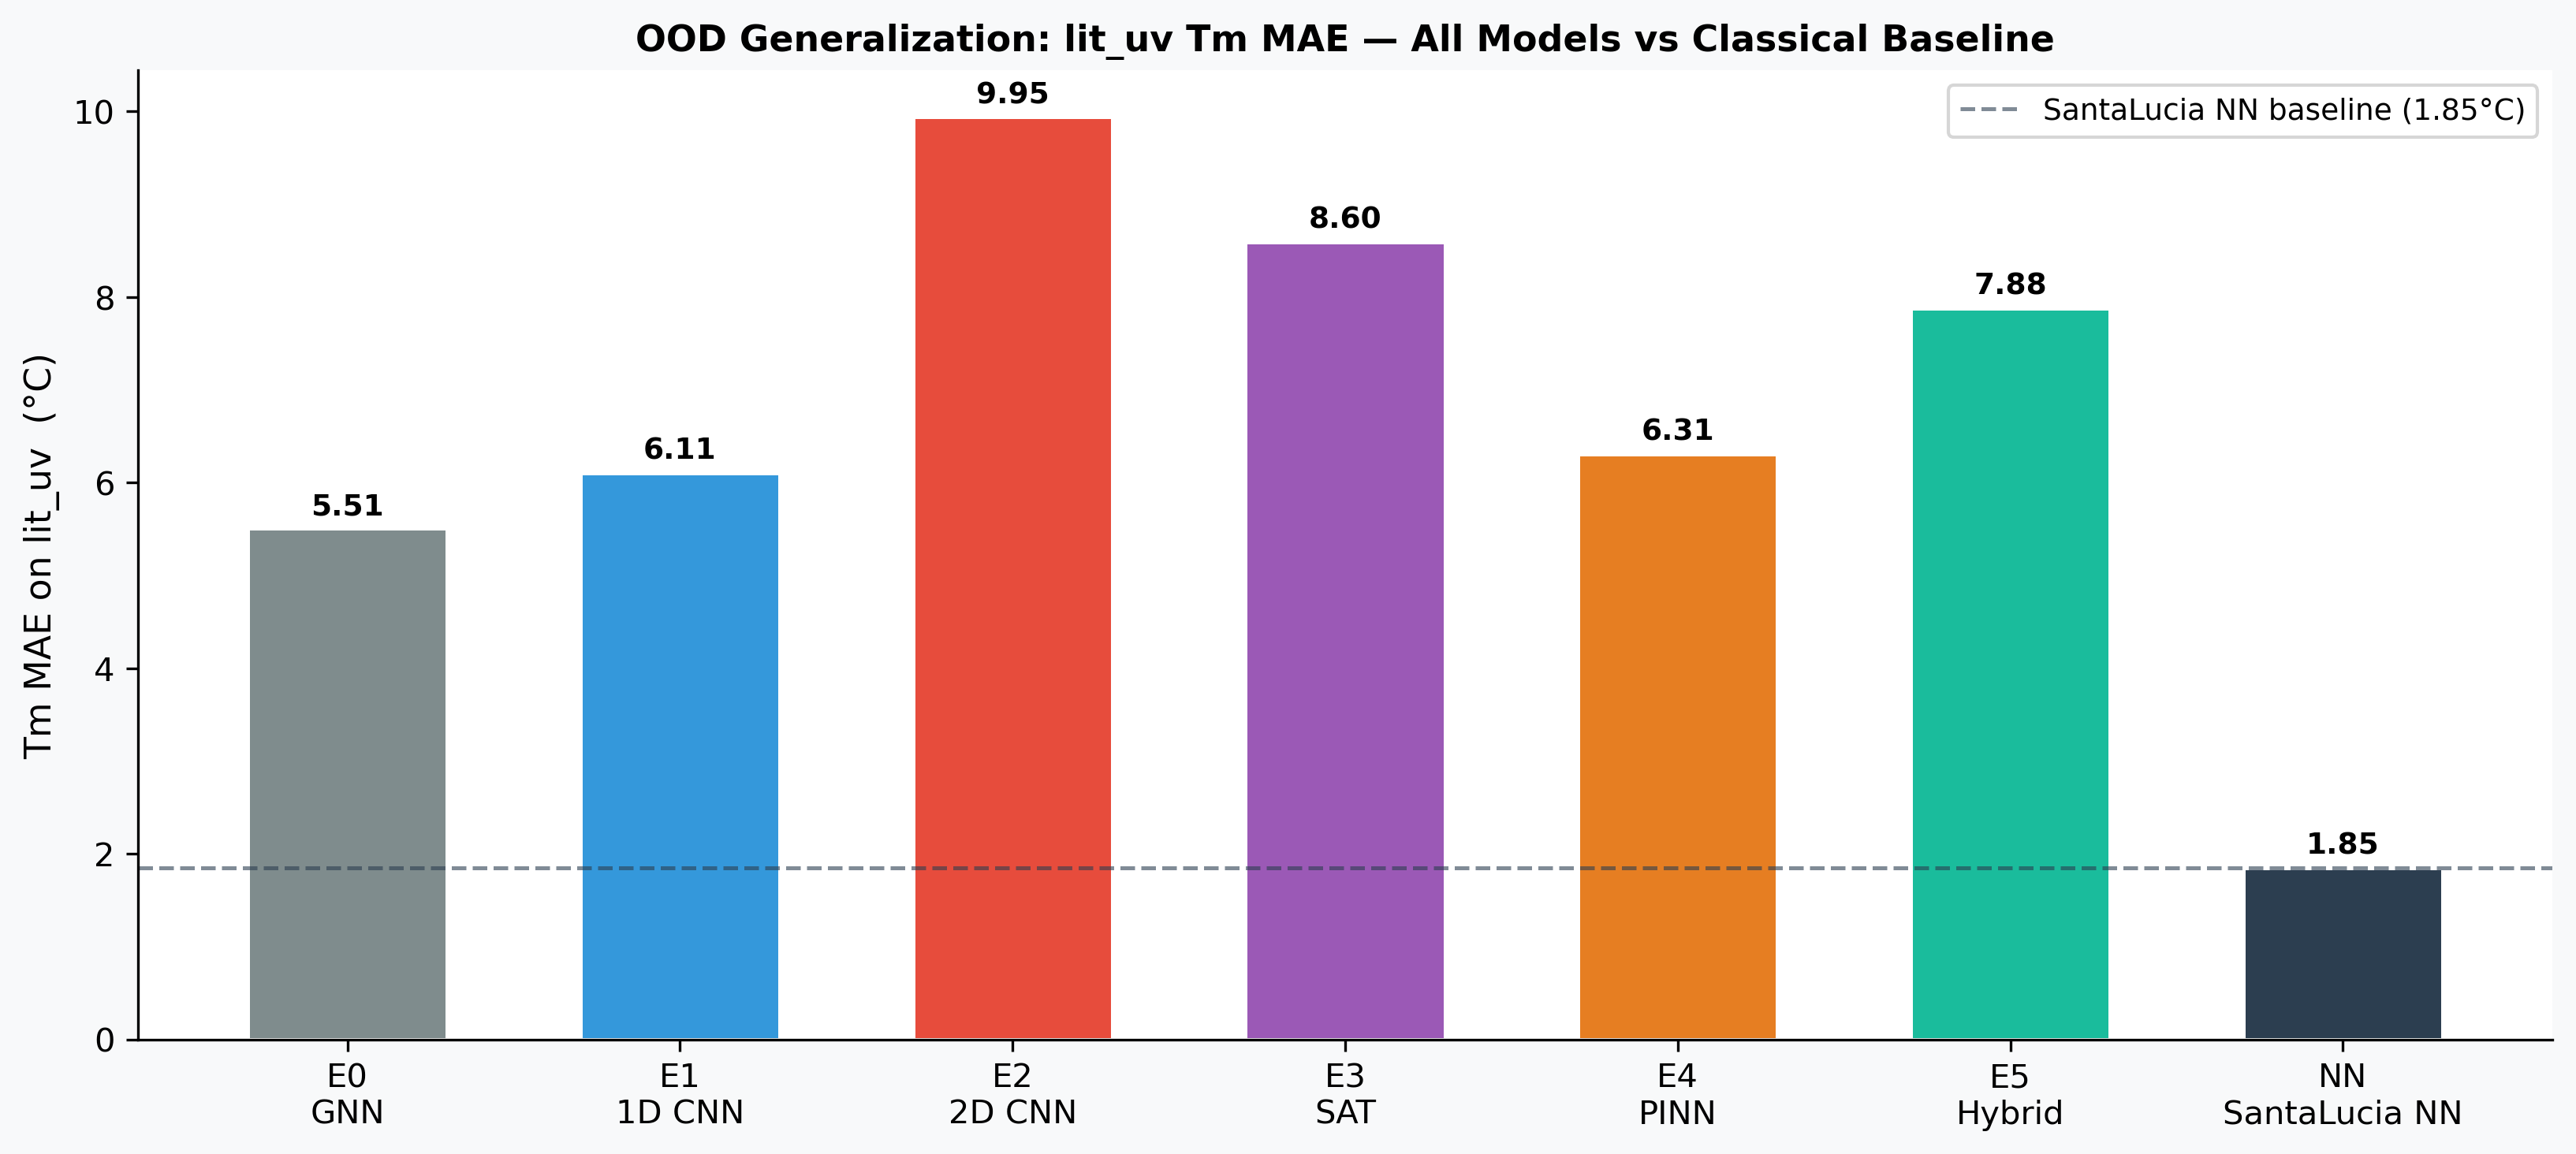
\includegraphics[width=0.90\textwidth]{lit_uv_mae_bar.png}
    \caption{Out-of-distribution $T_m$ MAE on \texttt{lit\_uv} for all six neural network models and the SantaLucia nearest-neighbor classical baseline (dashed reference line). All neural network models underperform the classical model on \texttt{lit\_uv}. The GNN (E0) generalizes best among the deep learning models on both external datasets, while the 2D CNN (E2) and Hybrid (E5) fail to generalize to the \texttt{ov} mismatch dataset (MAE $>$20$^\circ$C; not shown in this figure).}
    \label{fig:ood}
\end{figure}

\section{Generalization to Mismatch Duplexes (\texttt{ov})}

The \texttt{ov} dataset provides a qualitatively distinct OOD probe from \texttt{lit\_uv}. While \texttt{lit\_uv} sequences are all perfectly complementary Watson-Crick duplexes, 97.8\% of \texttt{ov} sequences contain at least one internal mismatch or bulge --- positions in the duplex that are unpaired, denoted by a dot (\texttt{.}) inside the dot-bracket stem. For example, the structure

\begin{center}
\texttt{(((((((((.(((((((((+))))))))).)))))))))},
\end{center}

\noindent represents a 19-base-pair duplex with a single mismatched position on each strand (position 9 from the 5$'$ end). The two datasets therefore probe complementary failure modes: \texttt{lit\_uv} tests transfer across experimental platforms and ionic conditions, while \texttt{ov} tests the model's ability to handle unpaired positions embedded within a duplex stem.

\subsection{GNN Generalizes Consistently Across Both Duplex Datasets}

The GNN (E0) achieves $T_m$ MAE of 5.27$^\circ$C on \texttt{ov} --- the best performance of any model and nearly identical to its \texttt{lit\_uv} score (5.59$^\circ$C). This consistency across two structurally different duplex datasets, one with perfect pairing and one dominated by mismatches, is the strongest evidence in this thesis that the graph inductive bias captures physically transferable thermodynamic information.

The reason is structural. In the GNN graph representation, a mismatched nucleotide (a dot in the dot-bracket notation) is a node with only backbone edges and no hydrogen-bond edges. The model has learned, from the training data, that nodes lacking hydrogen-bond connectivity contribute differently to thermodynamic stability than fully paired nodes. This distinction is encoded explicitly in the graph topology and transfers naturally to the \texttt{ov} sequences without any mismatch-specific training.

\subsection{Position-Sensitive Models Fail on \texttt{ov}}

The 1D CNN (E0, 20.46$^\circ$C) and Hybrid (E5, 21.06$^\circ$C) show catastrophic degradation on \texttt{ov}. These models encode sequences as fixed-length position-indexed tensors. A mismatched position receives the same structural channel encoding (\texttt{.} $\to$ channel 6) as a loop position in a hairpin. The model has no mechanism to distinguish a mismatch inside a duplex stem from an unpaired nucleotide in a hairpin loop, because both produce the same local feature vector. The position-specific filters learned on hairpin training data do not transfer to the different positional patterns of mismatch duplexes.

\section{The Inversion: In-Distribution vs.\ Out-of-Distribution}

The most striking result in this thesis is the inversion between in-distribution and out-of-distribution rankings. The 2D CNN (E2) achieves the second-best in-distribution $T_m$ MAE (1.57$^\circ$C) but the worst out-of-distribution MAE (9.95$^\circ$C). Conversely, the GNN (E0) is the worst in-distribution model (3.28$^\circ$C) but the best out-of-distribution deep learning model (5.51$^\circ$C).

This is not a numerical artifact. It reflects a fundamental difference in what each model has learned.

\subsection{Why the GNN Generalizes Better}

The GNN encodes the DNA molecule as a graph where the structural connectivity, backbone bonds and hydrogen bonds, is made explicit through edge features. When applied to a duplex sequence from the literature UV melting dataset, the graph structure changes (a duplex graph has no hairpin loop; instead, it has an additional backbone bond joining the two strands at the ``$+$'' position), but the fundamental representation remains physically meaningful: base-pair hydrogen bonds are still encoded as H-bond edges, backbone connectivity is still encoded as backbone edges.

In other words, the GNN's inductive bias is grounded in the actual physics of the molecule. It has learned that certain edge types (G--C hydrogen bonds, stacked dinucleotide pairs) are thermodynamically significant. When it encounters a duplex, it can apply the same learned physics to a graph that has the same type of edges.

\subsection{Why the 2D CNN Generalizes Worst}

The 2D Folded Ladder encoding was specifically designed for hairpins. The folding procedure, which places the 5$'$ arm in row 0, the reversed 3$'$ arm in row 2, and the H-bond pattern in row 1, is meaningful only for hairpin sequences. When applied to a duplex (which is what the literature UV melting dataset contains), the encoding produces a different visual pattern: there is no backbone turn column, and both strands occupy rows 0 and 2 respectively. The 2D CNN learned to recognize thermodynamically informative patterns in the hairpin-specific folded structure, and those patterns do not transfer straightforwardly to the duplex representation.

This is an instance of what is sometimes called \textit{shortcut learning}: the model found a representation that works extremely well within its training distribution but has captured features specific to the measurement or structural context rather than the underlying thermodynamic physics.

\subsection{The PINN Result and Physical Constraints}

The PINN (E4) achieves the second-best out-of-distribution performance (6.31$^\circ$C), substantially better than the Hybrid (7.88$^\circ$C), SAT (8.60$^\circ$C), and 2D CNN (9.95$^\circ$C). This is the most interpretable finding in the generalization results. By explicitly penalizing predictions that violate thermodynamic laws ($\Delta H < 0$, $\Delta S < 0$, $\Delta G_{37} < 0$), the PINN is forced to remain in a physically consistent region of the output space. When transferred to the literature UV melting context, predictions that would have drifted into physically impossible regions are suppressed, and the model remains roughly calibrated.

This result supports a general principle: for machine learning models in science, incorporating physical constraints even when they can be satisfied approximately by data-driven fitting tends to improve robustness to distribution shift.

\section{The SantaLucia Gap}

All six neural network models are outperformed by the SantaLucia classical model (1.85$^\circ$C) on the \texttt{lit\_uv} evaluation. This is important to discuss carefully. It is not simply a failure of the neural networks.

The literature UV melting sequences are \textit{duplexes}, while the neural networks were trained on \textit{hairpins}. These are different molecular topologies: hairpins have a loop, duplexes do not. The neural networks are being asked to generalize from one topology to another, which is a substantial domain shift. The SantaLucia model, on the other hand, was explicitly designed and parameterized for duplexes --- it has no topology-specific architectural bias, only topology-specific parameters.

The situation reverses on the \texttt{ov} mismatch dataset. The SantaLucia nearest-neighbor model achieves $T_m$ MAE of 9.94$^\circ$C on \texttt{ov}, with a systematic positive bias of $+$9.8$^\circ$C --- it overpredicts $T_m$ by nearly 10$^\circ$C on average because it treats every position as a perfectly paired Watson-Crick base pair and has no mechanism to account for the destabilization caused by mismatches. The GNN (E0), by contrast, achieves 5.27$^\circ$C on \texttt{ov} --- a 47\% reduction in MAE relative to the classical model, despite never having been trained on duplex mismatch data. This is the one context in this thesis where a neural network outperforms the SantaLucia baseline, and it is precisely the context where the classical model's structural assumptions break down.

A more fair comparison on \texttt{lit\_uv} would be to train the neural networks on duplex data and evaluate on the same set. That experiment is left for future work. What the current results establish is that: (i) in the absence of matched training data, the classical physics model generalizes more robustly to perfect duplexes; and (ii) for the structurally more complex case of mismatch-containing duplexes, the GNN's graph topology encoding provides better generalization than the nearest-neighbor additivity assumption. This contrast highlights that classical and neural models have complementary strengths that depend on the structural complexity of the target sequences.

\section{Final Model Comparison}

Figure~\ref{fig:comparison} shows the complete model comparison across all metrics.

\begin{figure}[h!]
    \centering
    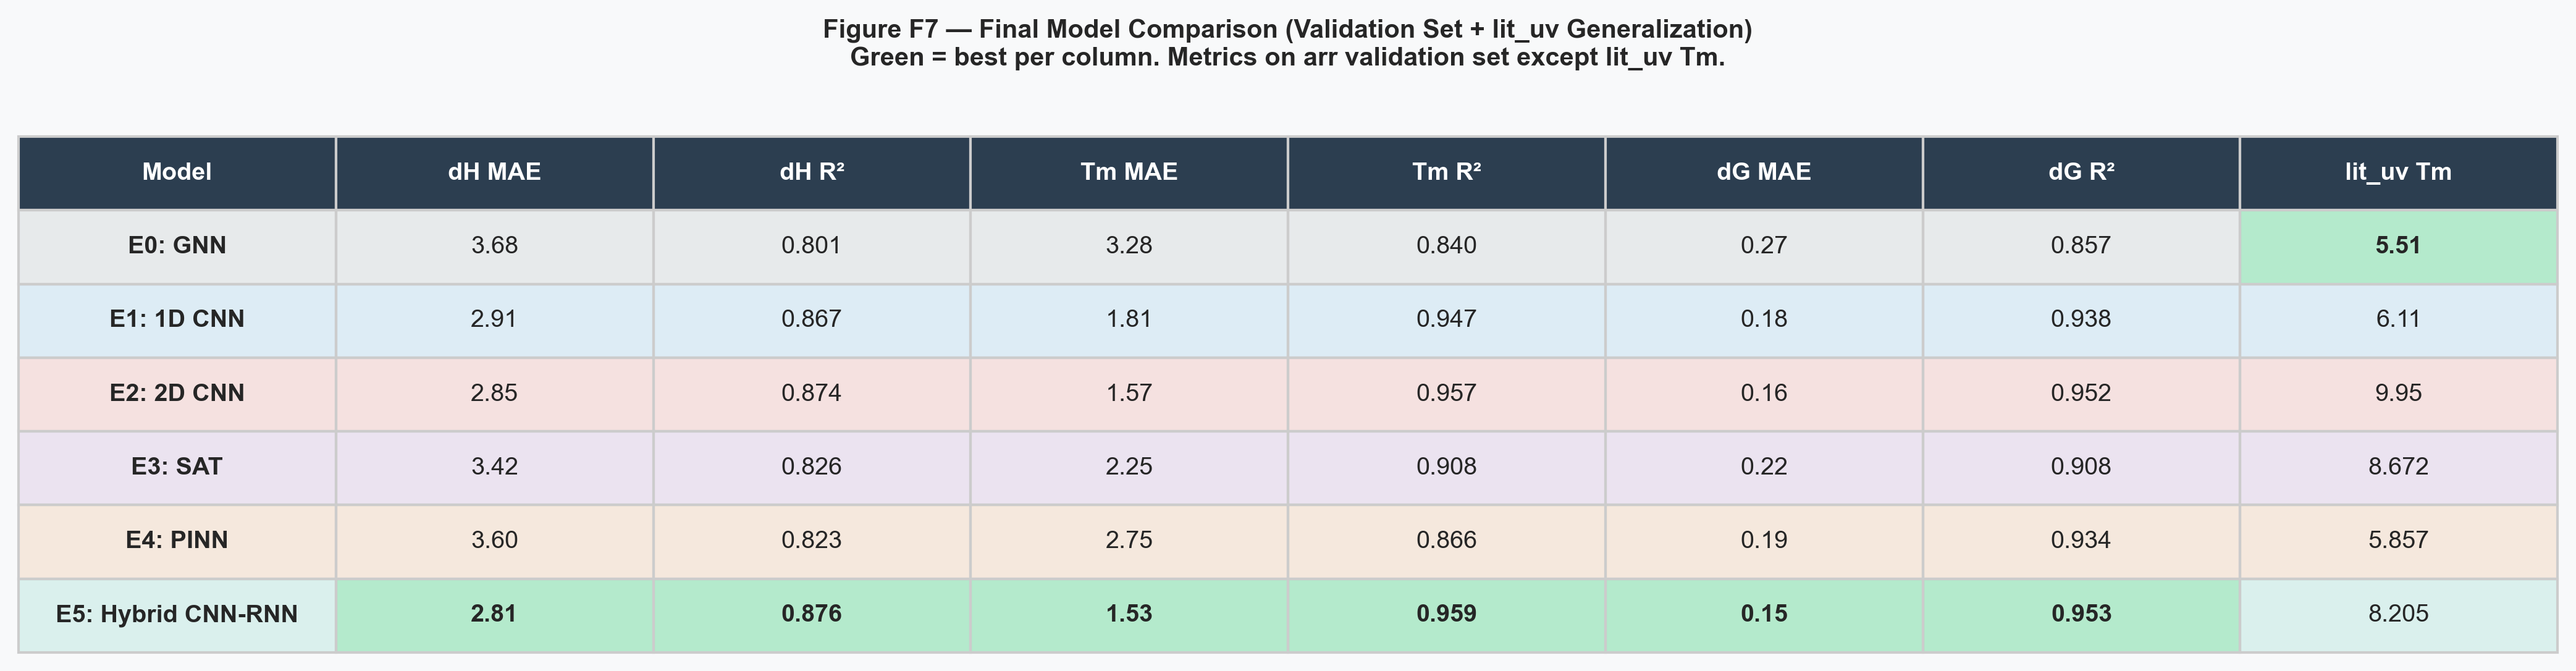
\includegraphics[width=\textwidth]{final_comparison_table.png}
    \caption{Complete comparison of all six models across all evaluation metrics: in-distribution $\Delta H$ MAE, $T_m$ MAE, $\Delta G_{37}$ MAE, $T_m$ $R^2$, and out-of-distribution lit\_uv $T_m$ MAE.}
    \label{fig:comparison}
\end{figure}

% =========================================================
\chapter{Conclusion}
% =========================================================

\section{Summary of Contributions}

This thesis investigated whether the choice of neural network inductive bias matters for predicting DNA oligonucleotide thermodynamics from the Array Melt dataset of Greenleaf et al. The answer is: yes, it matters substantially, and in ways that are not always intuitive.

The main findings are:

\begin{enumerate}
    \item \textbf{The 2D Folded Ladder encoding achieves competitive in-distribution performance.} By folding the hairpin sequence into a 2D matrix that places paired bases in adjacent rows, 2D convolutional filters can directly capture base-pair stacking interactions. The 2D CNN achieved $T_m$ MAE of 1.57$^\circ$C, outperforming the GNN baseline (3.28$^\circ$C) by a substantial margin on the array training distribution.

    \item \textbf{In-distribution performance does not predict out-of-distribution performance.} The 2D CNN, despite its in-distribution strength, generalized worst to external UV-melt duplex data. The GNN, the weakest in-distribution model, generalized best. This inversion is the central empirical finding of this thesis.

    \item \textbf{Physical constraints improve generalization.} The PINN (E4), by incorporating thermodynamic laws into the loss function, achieved the second-best out-of-distribution performance despite not being the best in-distribution model. This supports the value of physics-informed training for robustness to distribution shift.

    \item \textbf{The classical SantaLucia model remains a strong baseline on perfect duplex data, but the GNN outperforms it on mismatch duplexes.} All six neural networks underperformed the classical nearest-neighbor model on the 348 perfectly complementary \texttt{lit\_uv} sequences, highlighting the domain shift from hairpin training data. However, on the 2,775 mismatch-containing \texttt{ov} sequences --- where the nearest-neighbor model's additivity assumption breaks down and it overpredicts $T_m$ by $+$9.8$^\circ$C on average --- the GNN achieves a 47\% lower MAE (5.27$^\circ$C vs.\ 9.94$^\circ$C). This demonstrates that the graph inductive bias, which explicitly represents unpaired positions as nodes without hydrogen-bond edges, encodes thermodynamically relevant information that the classical model cannot capture.
\end{enumerate}

\section{Limitations}

There are several important limitations to this work. First, the out-of-distribution evaluation covers two external datasets (\texttt{lit\_uv}: 348 sequences; \texttt{ov}: 2,775 sequences), but both are duplex datasets. A more thorough evaluation across multiple external datasets with different structural types (e.g., hairpins with non-standard loop motifs, multi-branch junctions), sequence lengths, and ionic conditions would be needed to draw fully general conclusions. Second, the six models use the same hyperparameter settings and training budget; a model-specific hyperparameter search might change the relative rankings. Third, the \texttt{lit\_uv} test sequences are all duplexes while the training sequences are all hairpins, which means the OOD evaluation mixes domain shift with topology shift. Isolating these two factors would require a dedicated duplex training set.

\section{Future Work}

Several natural directions follow from this thesis:

\begin{itemize}
    \item \textbf{Duplex training:} Training the 2D CNN and Hybrid models on both hairpin and duplex data would directly test whether their poor generalization is due to the topology shift or the measurement shift.
    \item \textbf{Equivariant 2D encoding for duplexes:} Extending the Folded Ladder encoding to handle arbitrary structural topologies (internal loops, bulges, multi-branch junctions) would make it applicable as a general thermodynamic prediction framework.
    \item \textbf{Larger PINN study:} A systematic study of which physical constraints are most effective for thermodynamic generalization would help understand which thermodynamic laws are most useful as inductive biases.
    \item \textbf{Transfer learning:} Pre-training on the large hairpin dataset and fine-tuning on small duplex datasets might allow the 2D CNN to combine its strong in-distribution representation with better generalization.
    \item \textbf{Uncertainty quantification:} Adding calibrated uncertainty estimates (e.g., dropout-based or Bayesian) would make the models more useful for practical applications like primer design, where knowing when the model is likely to be wrong is as important as knowing when it is right.
\end{itemize}

\section{Closing Remarks}

The question at the heart of this thesis, which inductive bias best captures DNA thermodynamics, turned out to have a nuanced answer. For in-distribution prediction on the array measurement platform, spatial biases aligned with the hairpin folding geometry work best. For generalization across experimental platforms and molecular topologies, the permutation-equivariant graph bias and physical thermodynamic constraints work better. Getting both right simultaneously remains an open problem.

What is clear is that representation matters. How you choose to encode a DNA sequence fundamentally shapes what a neural network can and cannot learn about it. The 2D Folded Ladder encoding introduced in this thesis is one concrete answer to the question of how to encode DNA hairpin structure for machine learning, and the results suggest it is a useful one --- at least within the distribution it was designed for.

% ---------------------------------------------------------
% BIBLIOGRAPHY
% ---------------------------------------------------------
\clearpage
\begin{singlespace}
\begin{thebibliography}{99}
\addcontentsline{toc}{chapter}{Bibliography}
\setlength{\itemsep}{1em}

\bibitem{santalucia1998}
SantaLucia, J.\ Jr.\ (1998).
A unified view of polymer, dumbbell, and oligonucleotide DNA nearest-neighbor thermodynamics.
\textit{Proceedings of the National Academy of Sciences}, 95(4), 1460--1465.

\bibitem{santalucia2004}
SantaLucia, J.\ Jr., \& Hicks, D.\ (2004).
The thermodynamics of DNA structural motifs.
\textit{Annual Review of Biophysics and Biomolecular Structure}, 33, 415--440.

\bibitem{greenleaf2025}
Greenleaf, W.J., Marklund, E., et al.\ (2025).
High-throughput DNA melt measurements enable improved models of DNA folding thermodynamics.
\textit{Nature Communications}. DOI: 10.1038/s41467-025-60455-4.

\bibitem{oliveira2020}
Oliveira, L.F.A., et al.\ (2020).
Single, double, and triple mismatches in short DNA duplexes: A thermodynamic study.
\textit{Biophysical Journal}, 119(6), 1067--1080.

\bibitem{gilmer2017}
Gilmer, J., Schütt, K.T., et al.\ (2017).
Neural message passing for quantum chemistry.
\textit{Proceedings of the 34th International Conference on Machine Learning (ICML)}, PMLR 70, 1263--1272.

\bibitem{shi2021}
Shi, Y., et al.\ (2021).
Masked label prediction: Unified message passing model for semi-supervised classification.
\textit{IJCAI 2021}.

\bibitem{vinyals2016}
Vinyals, O., Bengio, S., \& Kudlur, M.\ (2016).
Order matters: Sequence to sequence for sets.
\textit{ICLR 2016}.

\bibitem{alipanahi2015}
Alipanahi, B., Delong, A., Weirauch, M.T., \& Frey, B.J.\ (2015).
Predicting the sequence specificities of DNA- and RNA-binding proteins by deep learning.
\textit{Nature Biotechnology}, 33(8), 831--838.

\bibitem{zhou2015}
Zhou, J., \& Troyanskaya, O.G.\ (2015).
Predicting effects of noncoding variants with deep sequence-based models.
\textit{Nature Methods}, 12(10), 931--934.

\bibitem{bronstein2021}
Bronstein, M.M., Bruna, J., Cohen, T., \& Veličković, P.\ (2021).
Geometric deep learning: Grids, groups, graphs, geodesics, and gauges.
\textit{arXiv preprint arXiv:2104.13478}.

\bibitem{raissi2019}
Raissi, M., Perdikaris, P., \& Karniadakis, G.E.\ (2019).
Physics-informed neural networks: A deep learning framework for solving forward and inverse problems involving nonlinear partial differential equations.
\textit{Journal of Computational Physics}, 378, 686--707.

\bibitem{zuker2003}
Zuker, M.\ (2003).
Mfold web server for nucleic acid folding and hybridization prediction.
\textit{Nucleic Acids Research}, 31(13), 3406--3415.

\bibitem{owczarzy2004}
Owczarzy, R., et al.\ (2004).
Effects of sodium ions on DNA duplex oligomers: Improved predictions of melting temperatures.
\textit{Biochemistry}, 43(12), 3537--3554.

\bibitem{vaswani2017}
Vaswani, A., et al.\ (2017).
Attention is all you need.
\textit{NeurIPS 2017}.

\bibitem{dnabert2021}
Ji, Y., et al.\ (2021).
DNABERT: Pre-trained bidirectional encoder representations from transformers model for DNA-language in genome.
\textit{Bioinformatics}, 37(15), 2112--2120.

\bibitem{nucleotidetransformer2023}
Dalla-Torre, H., et al.\ (2023).
The nucleotide transformer: Building and evaluating robust foundation models for human genomics.
\textit{bioRxiv}.

\bibitem{rnaFM2022}
Chen, J., et al.\ (2022).
Interpretable RNA foundation model from unannotated data for highly accurate RNA structure and function predictions.
\textit{arXiv preprint arXiv:2204.00300}.

\bibitem{kingma2015}
Kingma, D.P., \& Ba, J.\ (2015).
Adam: A method for stochastic optimization.
\textit{ICLR 2015}.

\bibitem{deepstabp}
Jung, F., et al.\ (2023).
DeepSTABp: A deep learning approach for the prediction of thermal protein stability.
\textit{International Journal of Molecular Sciences}, 24(8), 7444.

\bibitem{deepmel2020}
Minnoye, L., et al.\ (2020).
Cross-species analysis of enhancer logic using deep learning.
\textit{Genome Research}, 30(12), 1815--1834.

\bibitem{doench2016}
Doench, J.G., Fusi, N., Sullender, M., et al.\ (2016).
Optimized sgRNA design to maximize activity and minimize off-target effects of CRISPR-Cas9 nucleases.
\textit{Nature Biotechnology}, 34(2), 184--191. DOI: 10.1038/nbt.3437.

\bibitem{seeman2018}
Seeman, N.C., \& Sleiman, H.F.\ (2018).
DNA nanotechnology.
\textit{Nature Reviews Materials}, 3, 17068. DOI: 10.1038/natrevmats.2017.68.

\end{thebibliography}
\end{singlespace}

\end{document}
